%!TEX root = ../report.tex

\chapter{Evaluation}
%Implementation and measurements.
\newpage{}
\section{Test case 1}%
\label{sec:test_case_1}

4 experiments were performed starting at different time. This makes the evaluation unbiased of
the starting position of the obstacles. There is a single obstacle moving along y axis.  
Figure~\ref{fig:test_case_1_experiment_start} shows the start position and direction of the moving
obstacle for each experiment. The trajectory and the velocity of the moving obstacle is same for each
experiment as described in~\ref{sec:test_case_1_single_obstacle_single_room}.

\begin{figure}[H]
    \centering
    \begin{subfigure}[b]{0.50\linewidth}
        \centering
        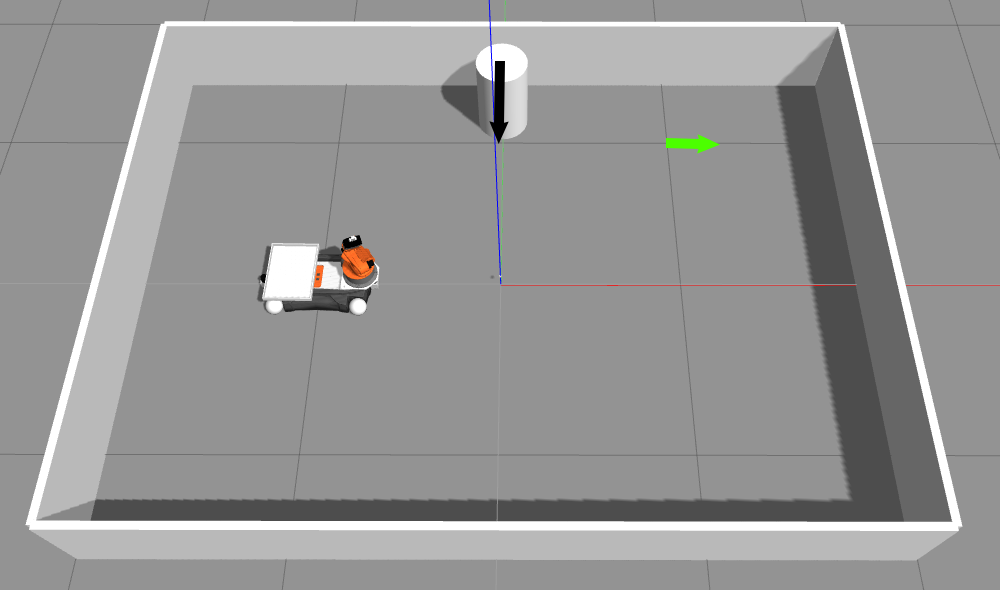
\includegraphics[width=0.95\textwidth]{images/test_case_1/exp1.png}
        \caption{Experiment 1}
    \end{subfigure}%
    \begin{subfigure}[b]{0.50\linewidth}
        \centering
        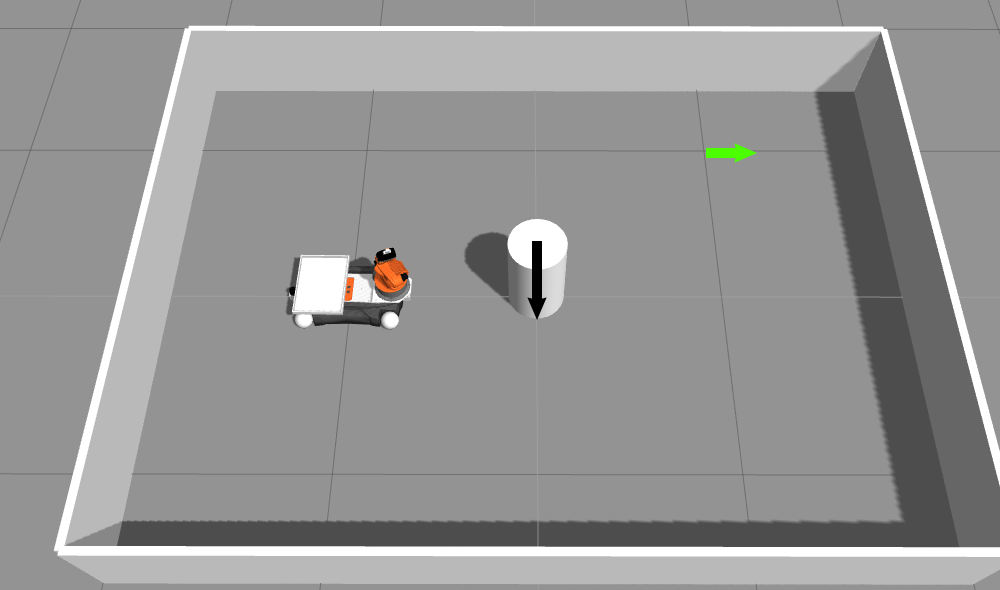
\includegraphics[width=0.95\textwidth]{images/test_case_1/exp2.png}
        \caption{Experiment 2}
    \end{subfigure}
    \begin{subfigure}[b]{0.50\linewidth}
        \centering
        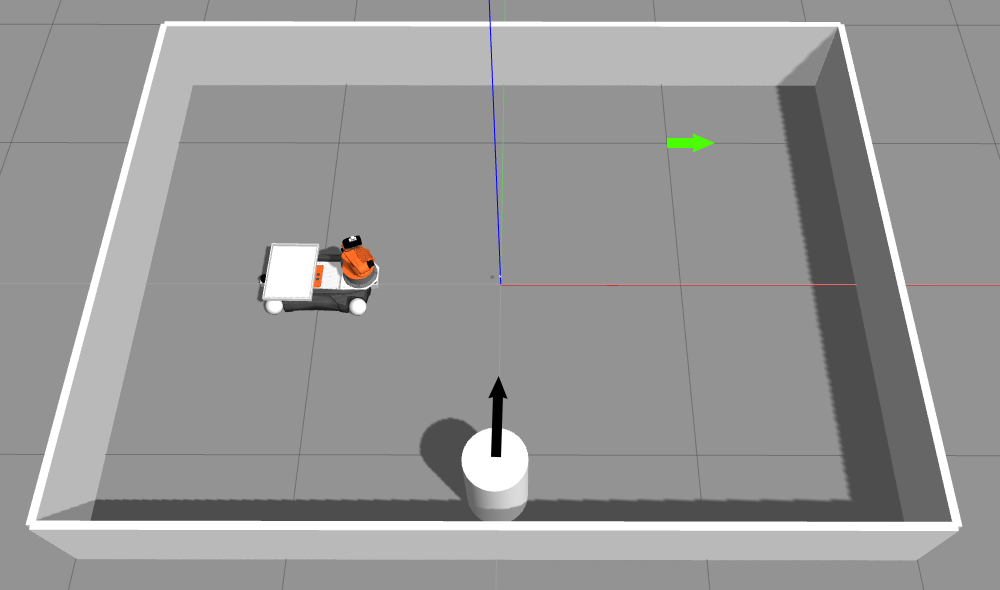
\includegraphics[width=0.95\textwidth]{images/test_case_1/exp3.png}
        \caption{Experiment 3}
    \end{subfigure}%
    \begin{subfigure}[b]{0.50\linewidth}
        \centering
        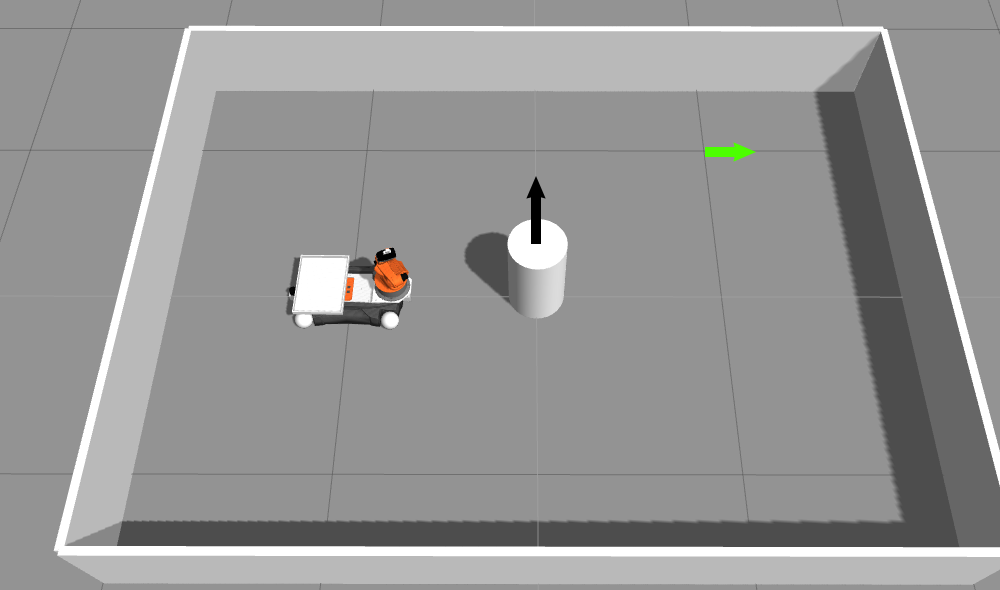
\includegraphics[width=0.95\textwidth]{images/test_case_1/exp4.png}
        \caption{Experiment 4}
    \end{subfigure}%
    \caption{Moving obstacle position and direction (black arrow) for experiments in test case 1.
    (Green arrow is goal position and orientation)}\label{fig:test_case_1_experiment_start}
\end{figure}

\subsection{TEB local planner}%
\label{sub:eval_teb_local_planner}

\begin{table}[H]
    \centering
    \begin{tabular}{cccc}
        \textbf{Experiment} & \textbf{Travel time} & \textbf{Re-plans} & \textbf{Collisions} \\\toprule
        static & 5.205 & 0 & 0 \\
             1 & 6.085 & 0 & 0 \\
             2 & 5.493 & 0 & 0 \\
             3 & 5.295 & 0 & 0 \\
             4 & 7.016 & 0 & 0 \\
    \end{tabular}
    \caption{Performance of teb local planner navigating in test case 1}\label{tab:perfomance_teb_test_case_1}
\end{table}

\begin{figure}[H]
    \centering
    \begin{subfigure}[b]{0.50\linewidth}
        \centering
        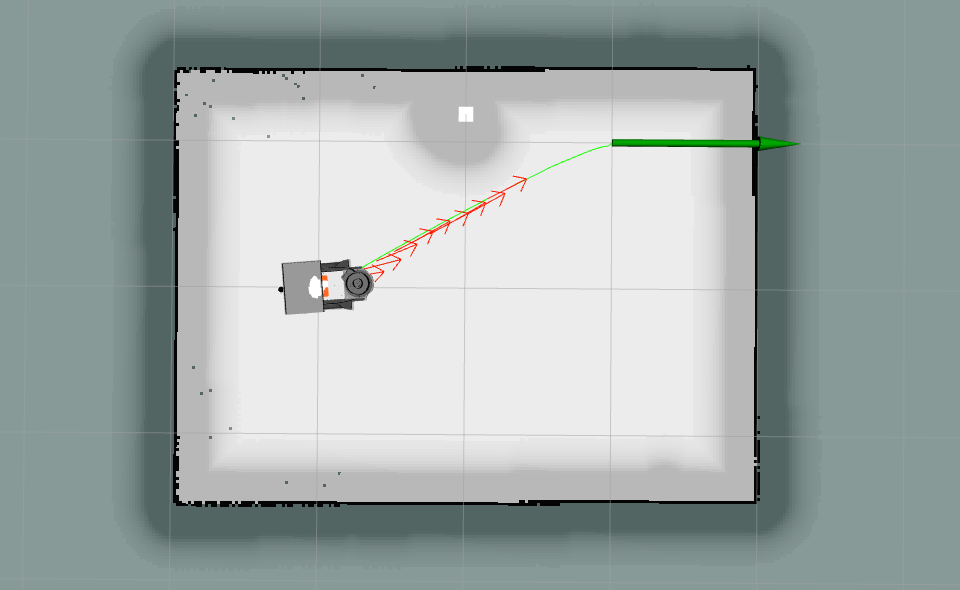
\includegraphics[width=0.95\textwidth]{images/teb_single_1_obs/1/5039.png}
        \caption{t=0.39s}
    \end{subfigure}%
    \begin{subfigure}[b]{0.50\linewidth}
        \centering
        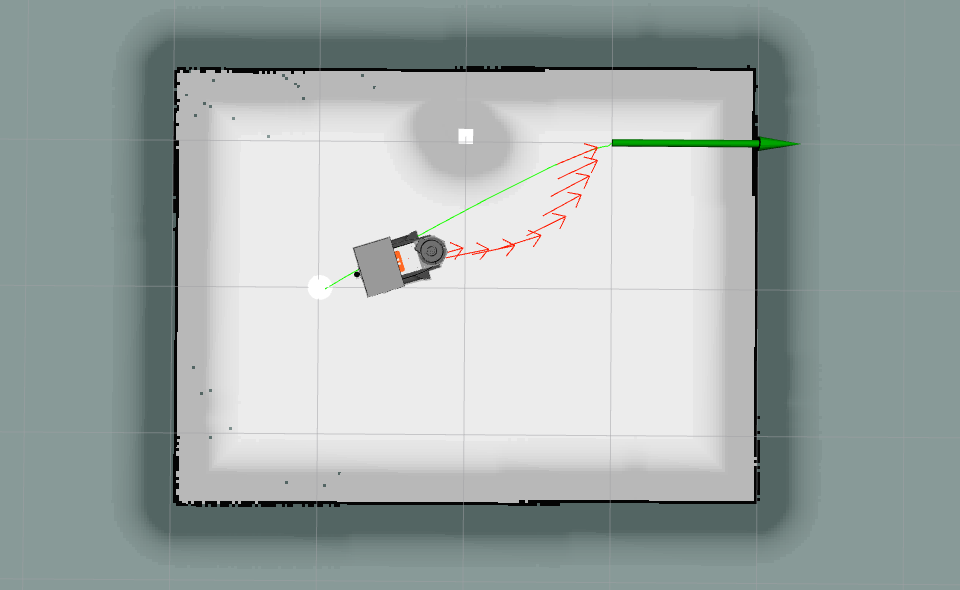
\includegraphics[width=0.95\textwidth]{images/teb_single_1_obs/1/5158.png}
        \caption{t=1.58s}
    \end{subfigure}
    \begin{subfigure}[b]{0.50\linewidth}
        \centering
        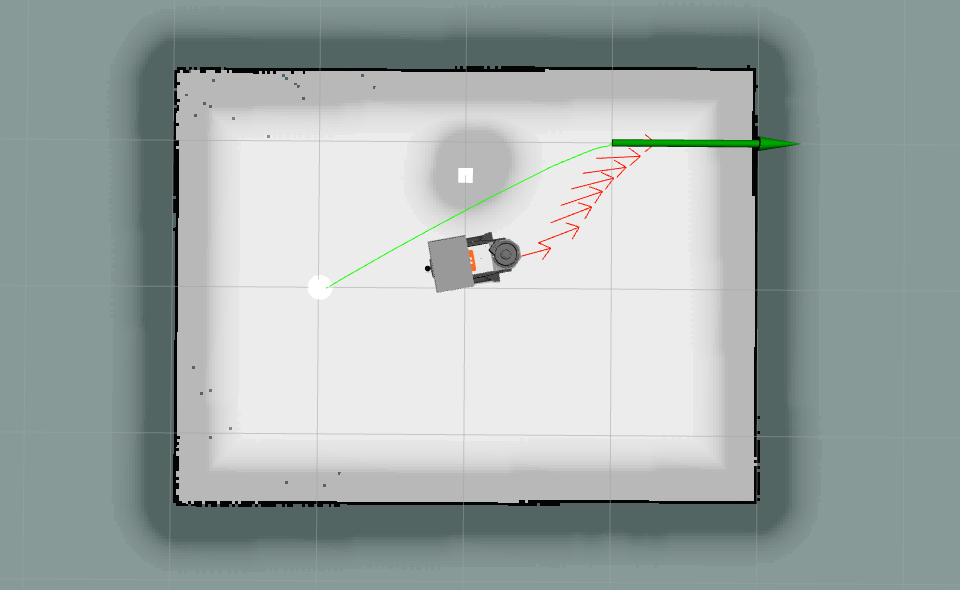
\includegraphics[width=0.95\textwidth]{images/teb_single_1_obs/1/5267.png}
        \caption{t=2.67s}
    \end{subfigure}%
    \begin{subfigure}[b]{0.50\linewidth}
        \centering
        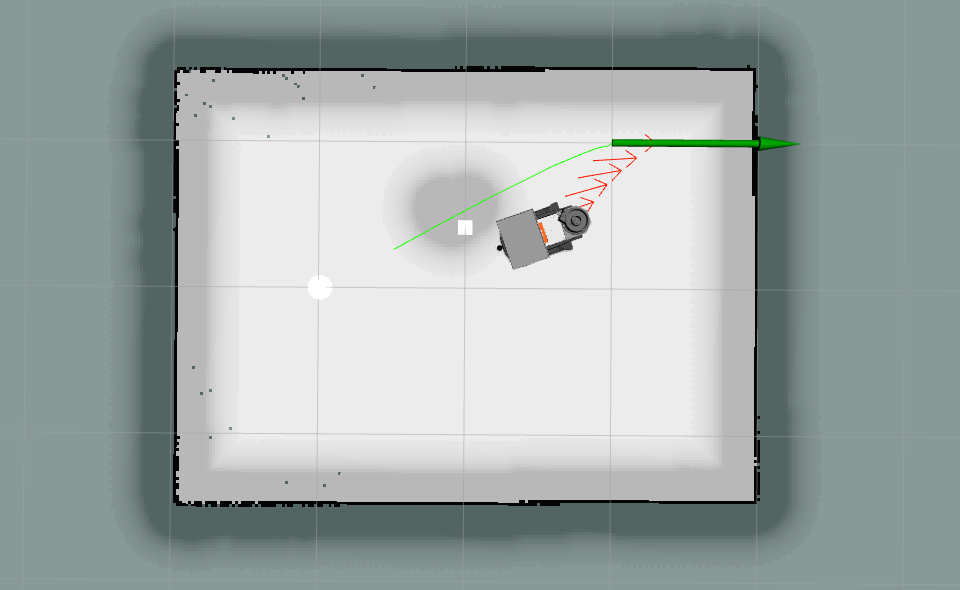
\includegraphics[width=0.95\textwidth]{images/teb_single_1_obs/1/5381.png}
        \caption{t=3.81s}
    \end{subfigure}
    \caption{teb local planner navigating in test case 1 (experiment 1) (Line in green is
        global path, red arrows are local planner's path, white square is the obstacle and green arrow
        is the position of goal)}\label{fig:teb_test_case_1_exp_1}
\end{figure}

\subsection{Spline based planner}%
\label{sub:eval_spline_based_planner}

\begin{table}[H]
    \centering
    \begin{tabular}{cccc}
        \textbf{Experiment} & \textbf{Travel time} & \textbf{Re-plans} & \textbf{Collisions} \\\toprule
        static & 5.421 & 0 & 0 \\
             1 & 5.958 & 0 & 0 \\
             2 & 5.347 & 0 & 0 \\
             3 & 5.326 & 0 & 0 \\
             4 & 5.664 & 0 & 0 \\
    \end{tabular}
    \caption{Performance of spline based planner navigating in test case 1}\label{tab:perfomance_spline_test_case_1}
\end{table}

\begin{figure}[ht]
    \centering
    \begin{subfigure}[b]{0.30\linewidth}
        \centering
        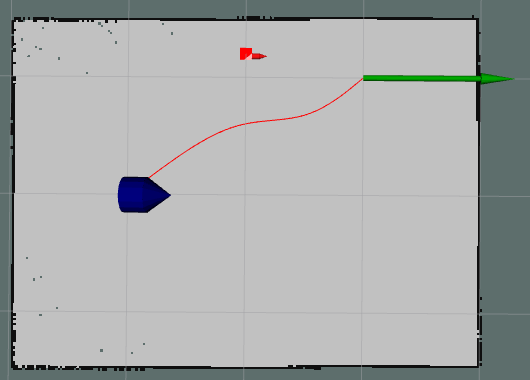
\includegraphics[width=0.95\textwidth]{images/spline_single_1_obs/1/5003.png}
        \caption{t=0.03s}
    \end{subfigure}%
    \begin{subfigure}[b]{0.30\linewidth}
        \centering
        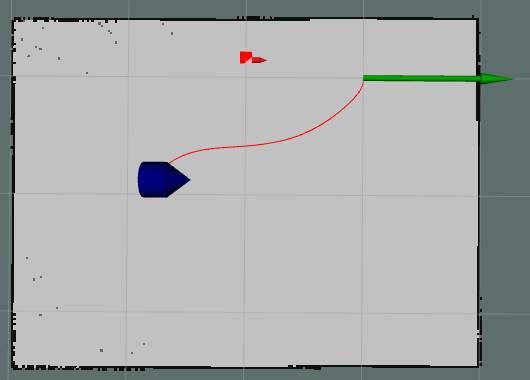
\includegraphics[width=0.95\textwidth]{images/spline_single_1_obs/1/5068.png}
        \caption{t=0.68}
    \end{subfigure}%
    \begin{subfigure}[b]{0.30\linewidth}
        \centering
        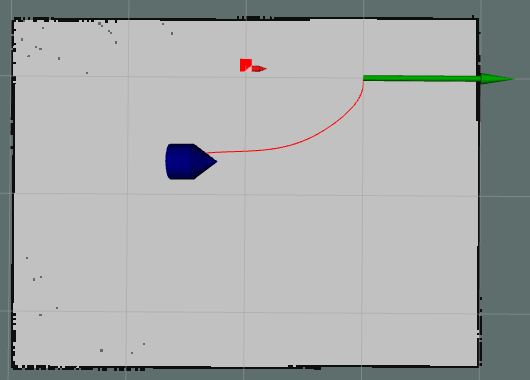
\includegraphics[width=0.95\textwidth]{images/spline_single_1_obs/1/5126.png}
        \caption{t=1.26s}
    \end{subfigure}
    \begin{subfigure}[b]{0.30\linewidth}
        \centering
        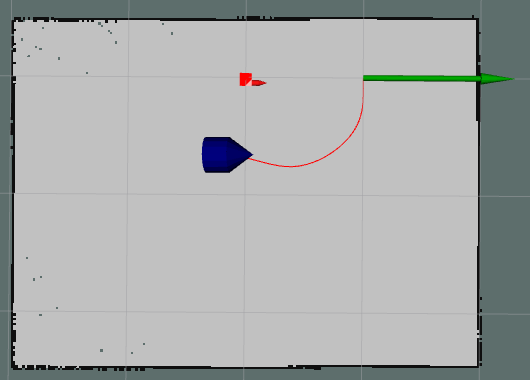
\includegraphics[width=0.95\textwidth]{images/spline_single_1_obs/1/5190.png}
        \caption{t=1.90s}
    \end{subfigure}%
    \begin{subfigure}[b]{0.30\linewidth}
        \centering
        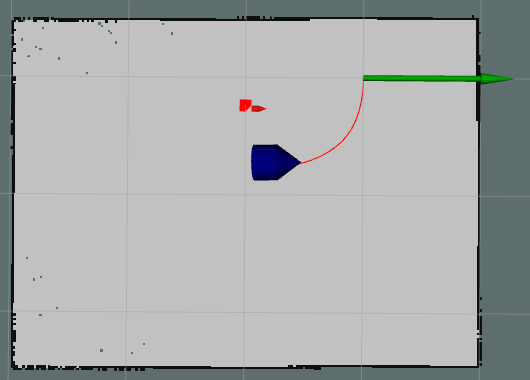
\includegraphics[width=0.95\textwidth]{images/spline_single_1_obs/1/5277.png}
        \caption{t=2.77s}
    \end{subfigure}%
    \begin{subfigure}[b]{0.30\linewidth}
        \centering
        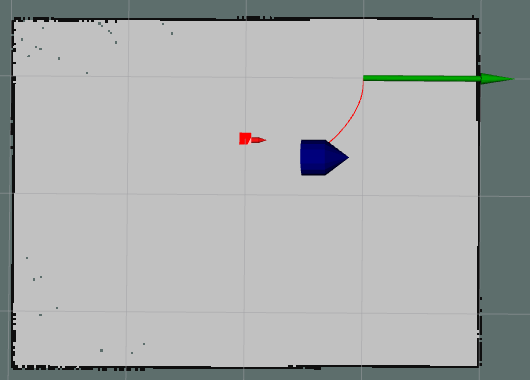
\includegraphics[width=0.95\textwidth]{images/spline_single_1_obs/1/5365.png}
        \caption{t=3.65s}
    \end{subfigure}
    \caption{Spline based planner navigating in test case 1 (experiment 1) (red line is motion
    planner's path, red square is moving obstacle and green arrow is goal position)}\label{fig:spline_test_case_1_exp_1}
\end{figure}

\subsection{DWA planner}%
\label{sub:eval_dwa_planner}

\begin{table}[H]
    \centering
    \begin{tabular}{cccc}
        \textbf{Experiment} & \textbf{Travel time} & \textbf{Re-plans} & \textbf{Collisions} \\\toprule
        static & 19.526 & 0 & 0 \\
             1 & 20.064 & 0 & 0 \\
             2 & 20.887 & 0 & 0 \\
             3 & 15.935 & 0 & 0 \\
             4 & 13.614 & 0 & 0 \\
    \end{tabular}
    \caption{Performance of DWA planner navigating in test case 1}\label{tab:perfomance_dwa_test_case_1}
\end{table}

\begin{figure}[ht]
    \centering
    \begin{subfigure}[b]{0.30\linewidth}
        \centering
        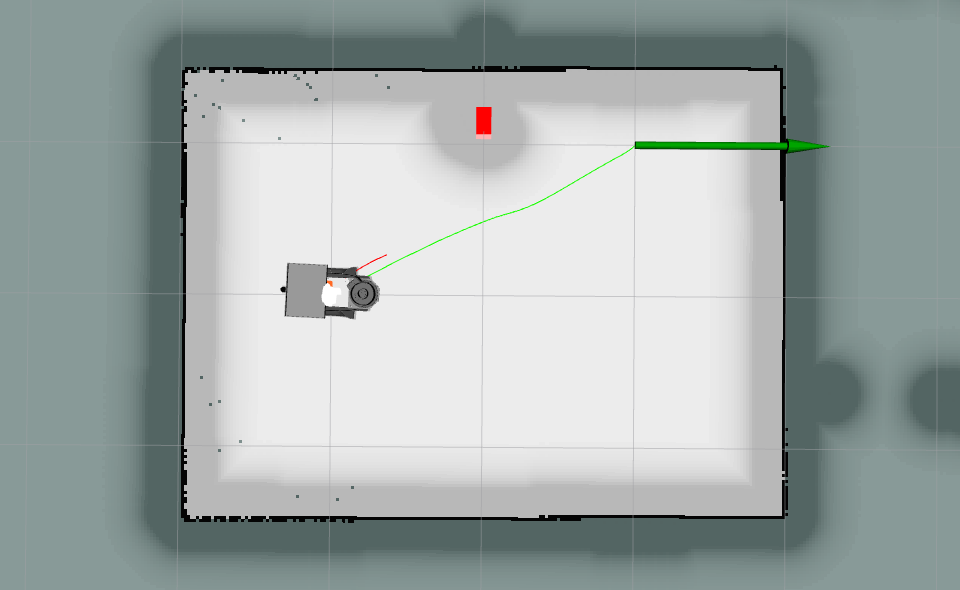
\includegraphics[width=0.95\textwidth]{images/dwa_single_1_obs/1/5027.png}
        \caption{t=0.27s}
    \end{subfigure}%
    \begin{subfigure}[b]{0.30\linewidth}
        \centering
        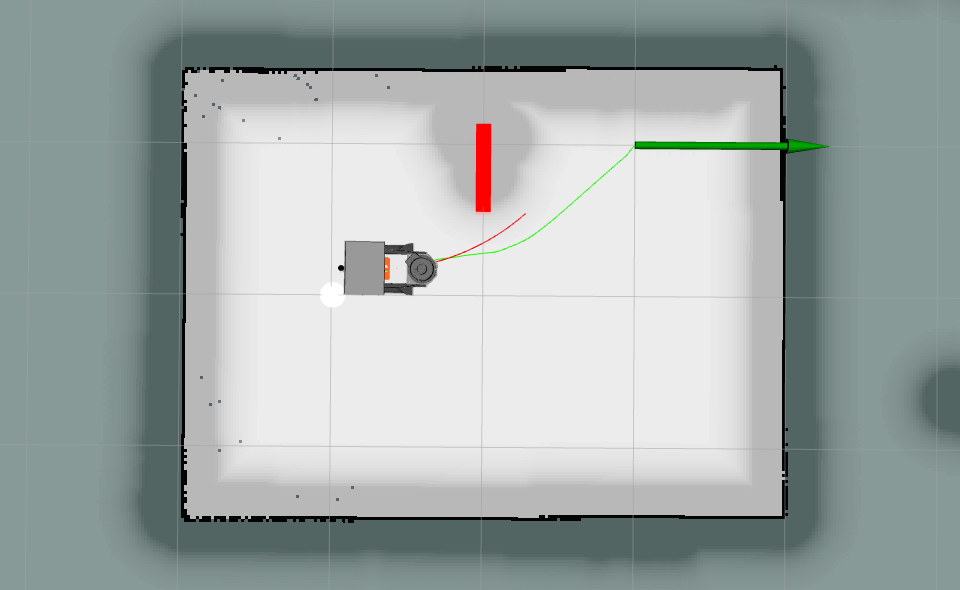
\includegraphics[width=0.95\textwidth]{images/dwa_single_1_obs/1/5130.png}
        \caption{t=1.30s}
    \end{subfigure}%
    \begin{subfigure}[b]{0.30\linewidth}
        \centering
        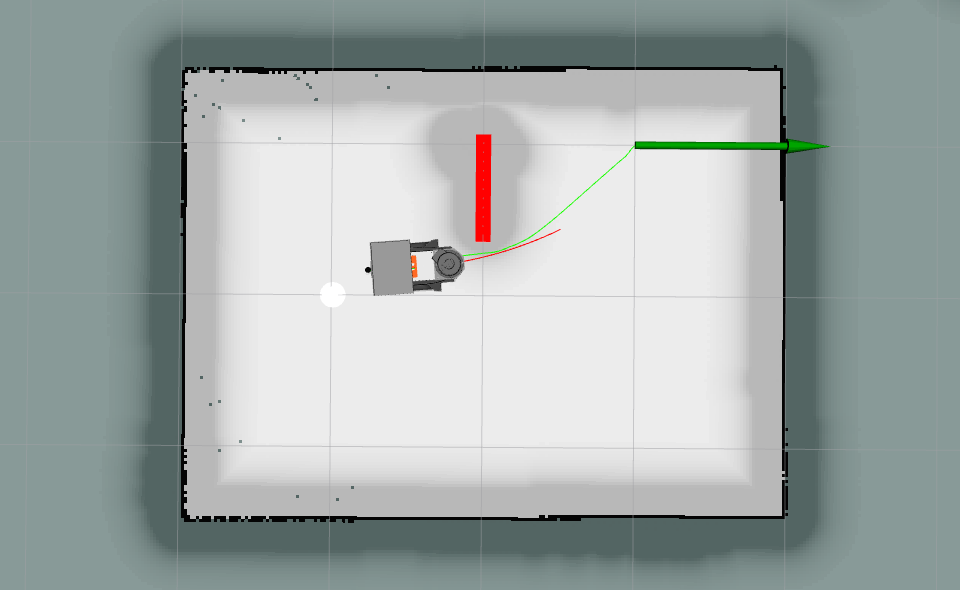
\includegraphics[width=0.95\textwidth]{images/dwa_single_1_obs/1/5167.png}
        \caption{t=1.67s}
    \end{subfigure}
    \begin{subfigure}[b]{0.30\linewidth}
        \centering
        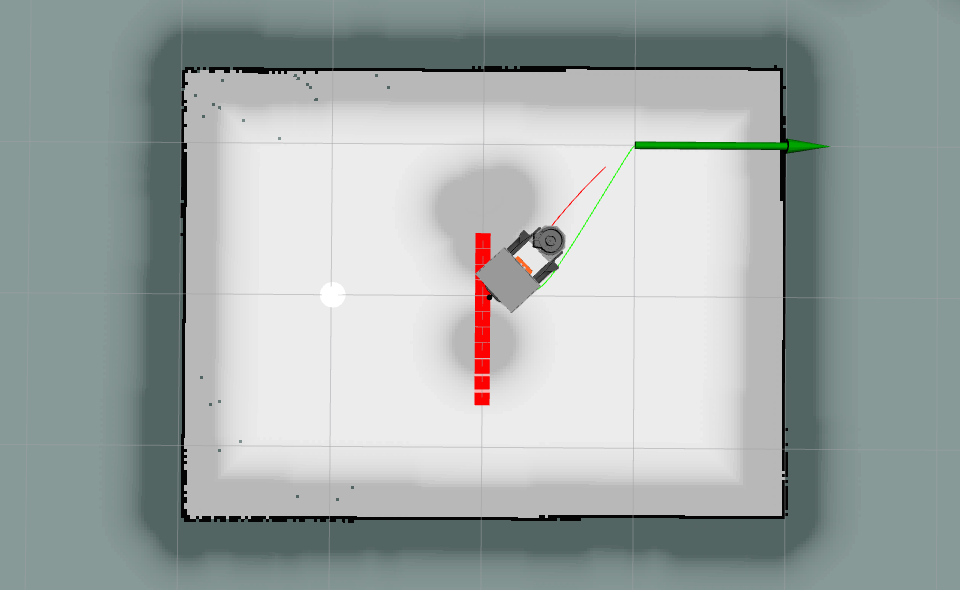
\includegraphics[width=0.95\textwidth]{images/dwa_single_1_obs/1/5396.png}
        \caption{t=3.96s}
    \end{subfigure}%
    \begin{subfigure}[b]{0.30\linewidth}
        \centering
        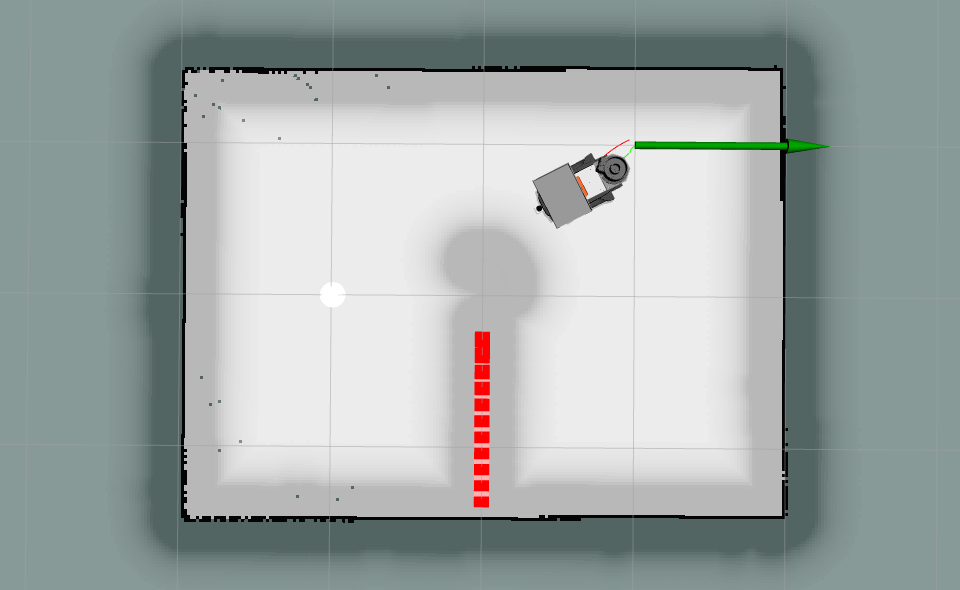
\includegraphics[width=0.95\textwidth]{images/dwa_single_1_obs/1/5580.png}
        \caption{t=5.80s}
    \end{subfigure}%
    \begin{subfigure}[b]{0.30\linewidth}
        \centering
        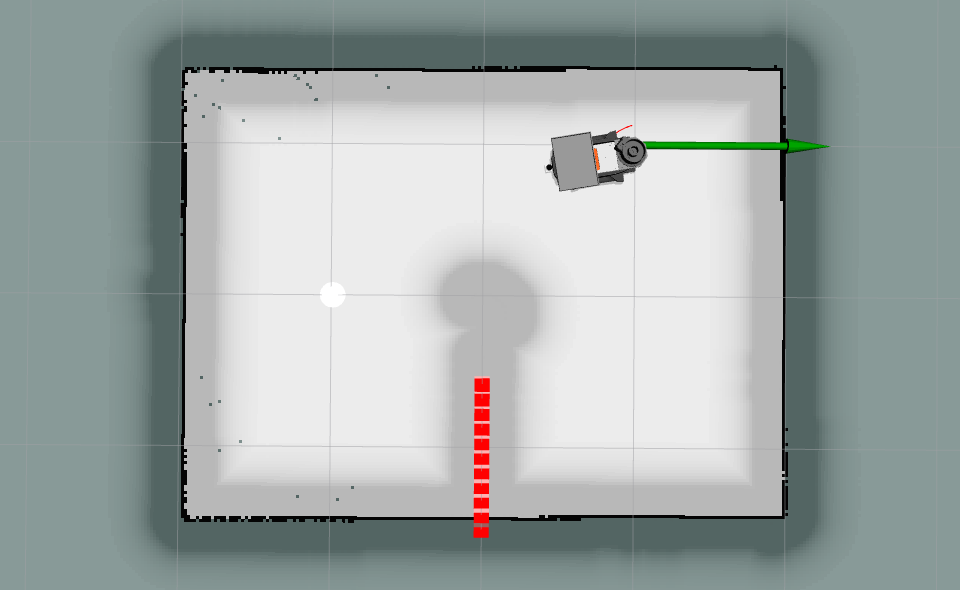
\includegraphics[width=0.95\textwidth]{images/dwa_single_1_obs/1/5667.png}
        \caption{t=6.67s}
    \end{subfigure}%
    \caption{DWA planner navigating in test case 1 (experiment 1) (Red squares are obstacle and the
    fake obstacles created by \texttt{obs\_to\_costmap}, green line is global path, red line is 
    local path generated by DWA and green arrow is goal position)}\label{fig:dwa_test_case_exp_1}
\end{figure}

\subsection{EBand planner}%
\label{sub:eval_eband_planner}

\begin{table}[H]
    \centering
    \begin{tabular}{cccc}
        \textbf{Experiment} & \textbf{Travel time} & \textbf{Re-plans} & \textbf{Collisions} \\\toprule
        static & 6.270 & 0 & 0 \\
             1 & 8.230 & 0 & 1 \\
             2 & 6.034 & 0 & 0 \\
             3 & 6.309 & 0 & 0 \\
             4 & 5.705 & 1 & 0 \\
    \end{tabular}
    \caption{Performance of EBand planner navigating in test case 1}\label{tab:perfomance_eband_test_case_1}
\end{table}

Images at various times for the first experiment are shown in Figure~\ref{fig:eband_test_case_1_exp_1}.
The collision is shown in Figure~\ref{subfig:eband_test_case_1_exp_1_collision}. We note that before
the collision occurred, the obstacle was in blind spot of the robot (refer~\ref{sec:setup}) as shown in Figure~\ref{subfig:eband_test_case_1_exp_1_blindspot}.
This changes the planners path from a previous curve avoiding obstacle (Figure~\ref{subfig:eband_test_case_1_exp_1_curve}) to a straight
line towards goal (Figure~\ref{subfig:eband_test_case_1_exp_1_blindspot}). This happens because the EBand planner
does not reason about the future. So, when an obstacle is in a blind spot of the robot, the planner 
believes that the obstacle no longer exists.

\begin{figure}[H]
    \centering
    \begin{subfigure}[b]{0.30\linewidth}
        \centering
        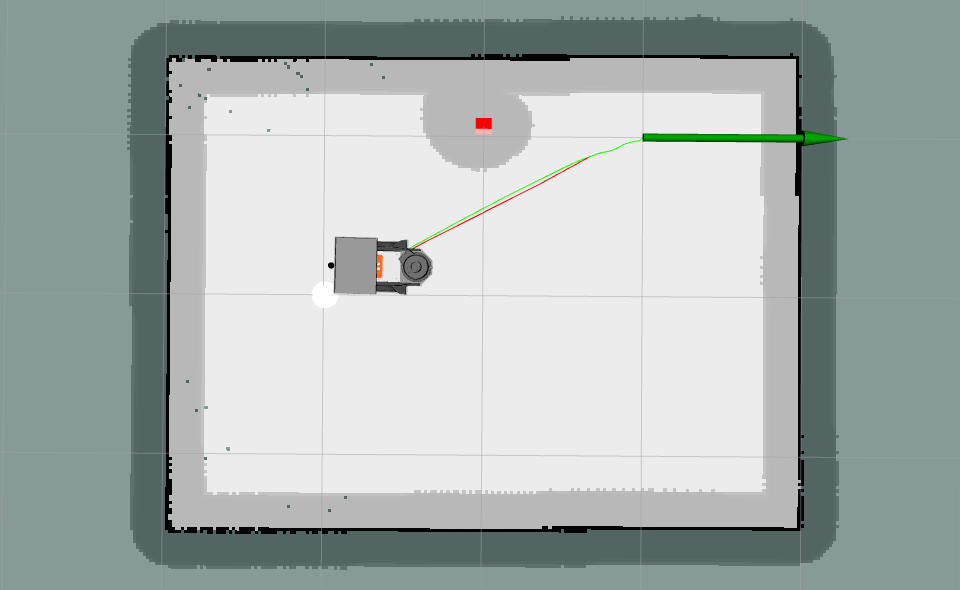
\includegraphics[width=0.95\textwidth]{images/eband_single_1_obs/1/3143.png} \caption{t=1.43s}
    \end{subfigure}%
    \begin{subfigure}[b]{0.30\linewidth}
        \centering
        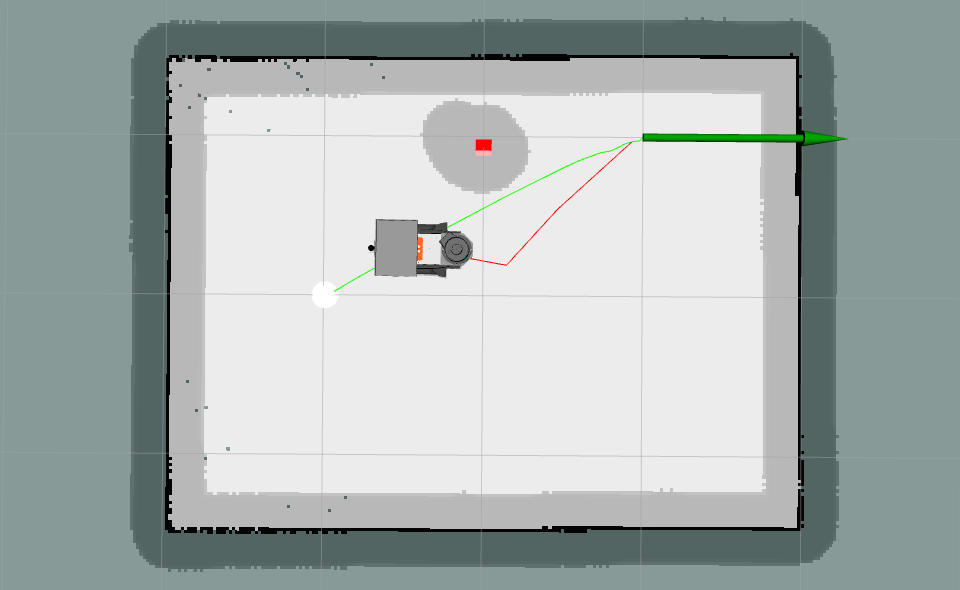
\includegraphics[width=0.95\textwidth]{images/eband_single_1_obs/1/3208.png} \caption{t=2.08s}\label{subfig:eband_test_case_1_exp_1_curve}
    \end{subfigure}%
    \begin{subfigure}[b]{0.30\linewidth}
        \centering
        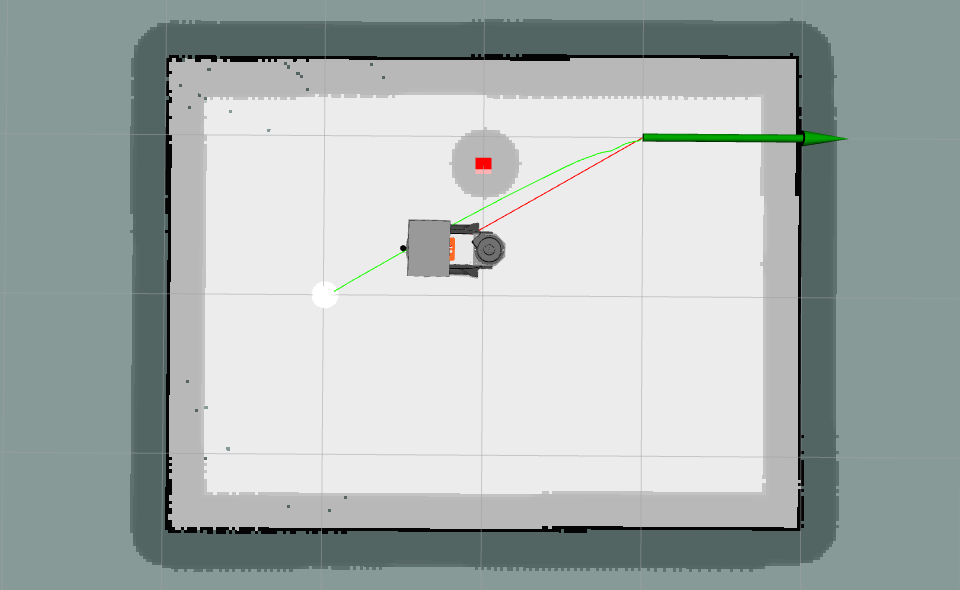
\includegraphics[width=0.95\textwidth]{images/eband_single_1_obs/1/3252.png} \caption{t=2.52s}\label{subfig:eband_test_case_1_exp_1_blindspot}
    \end{subfigure}
    \begin{subfigure}[b]{0.30\linewidth}
        \centering
        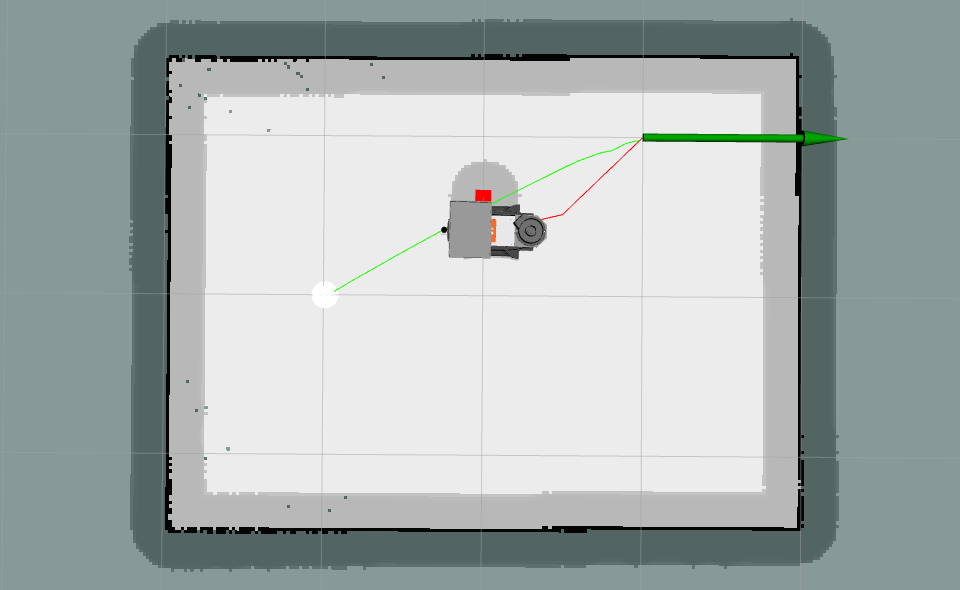
\includegraphics[width=0.95\textwidth]{images/eband_single_1_obs/1/3322.png} \caption{t=3.22s}\label{subfig:eband_test_case_1_exp_1_collision}
    \end{subfigure}%
    \begin{subfigure}[b]{0.30\linewidth}
        \centering
        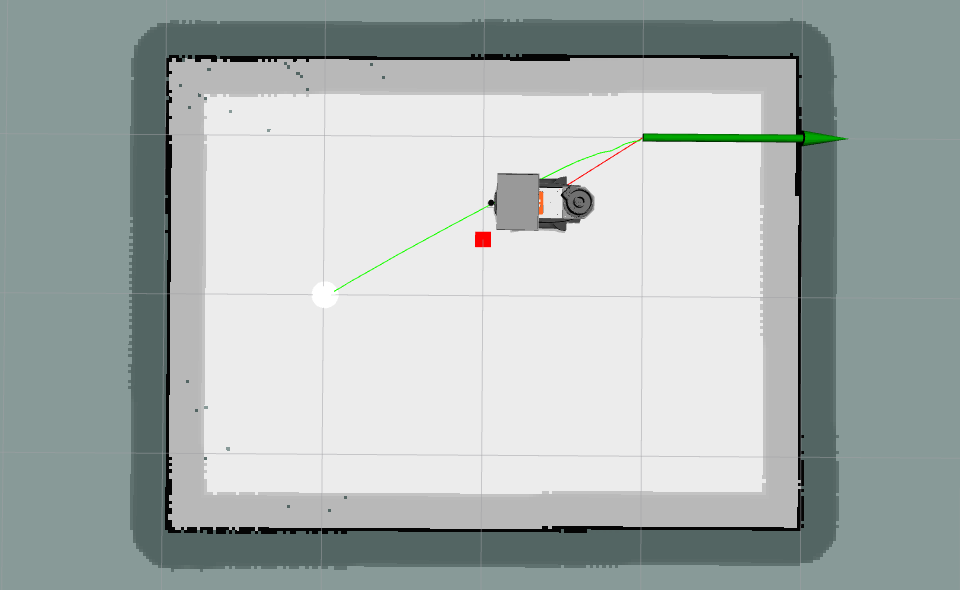
\includegraphics[width=0.95\textwidth]{images/eband_single_1_obs/1/3400.png} \caption{t=4.00s}
    \end{subfigure}%
    \begin{subfigure}[b]{0.30\linewidth}
        \centering
        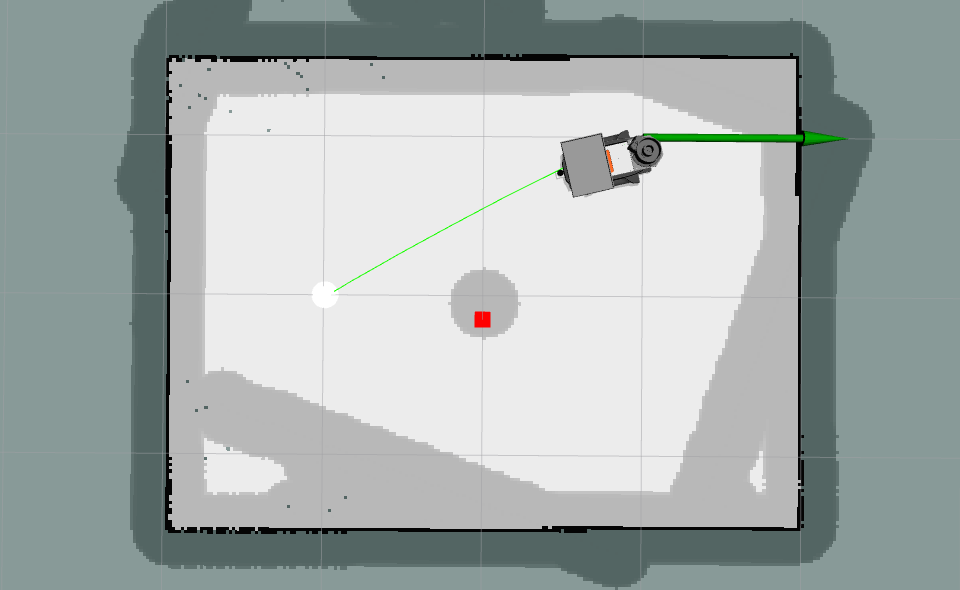
\includegraphics[width=0.95\textwidth]{images/eband_single_1_obs/1/3538.png} \caption{t=5.38s}
    \end{subfigure}
    \caption{EBand planner navigating in test case 1 (experiment 1) (green line is global path, 
    red line is Eband's plan, red square is moving obstacle and green arrow is goal)}\label{fig:eband_test_case_1_exp_1}
\end{figure}

\subsection{EBand2 planner}%
\label{sub:eval_eband2_planner}

\begin{table}[H]
    \centering
    \begin{tabular}{cccc}
        \textbf{Experiment} & \textbf{Travel time} & \textbf{Re-plans} & \textbf{Collisions} \\\toprule
        static & 6.270 & 0 & 0 \\
             1 & 5.814 & 1 & 0 \\
             2 & 5.884 & 0 & 0 \\
             3 & 5.718 & 0 & 0 \\
             4 & 6.684 & 1 & 0 \\
    \end{tabular}
    \caption{Performance of EBand2 planner navigating in test case 1}\label{tab:perfomance_eband2_test_case_1}
\end{table}

\begin{figure}[H]
    \centering
    \begin{subfigure}[b]{0.30\linewidth}
        \centering
        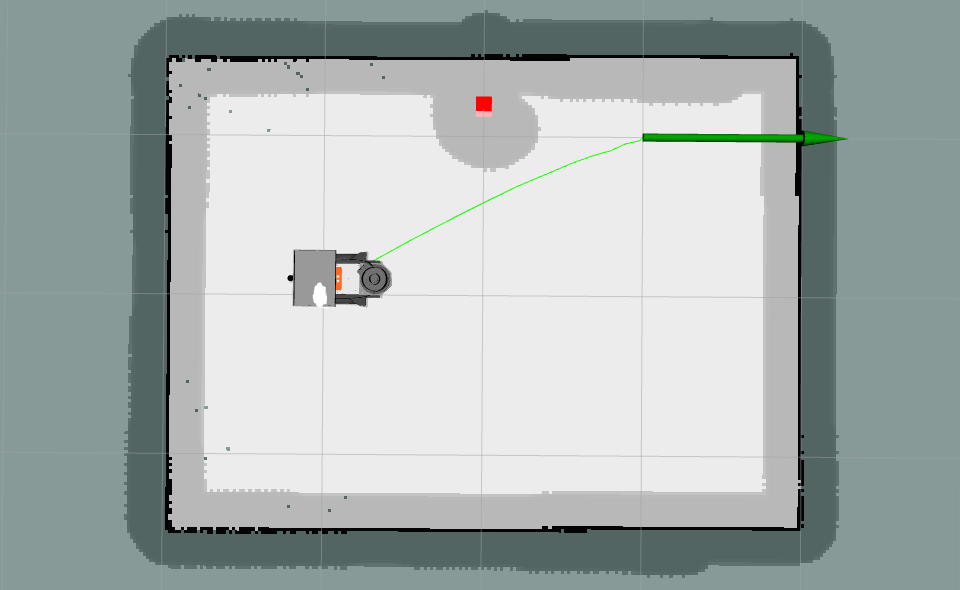
\includegraphics[width=0.95\textwidth]{images/eband_2_single_1_obs/1/5006.png} \caption{t=0.06s}
    \end{subfigure}%
    \begin{subfigure}[b]{0.30\linewidth}
        \centering
        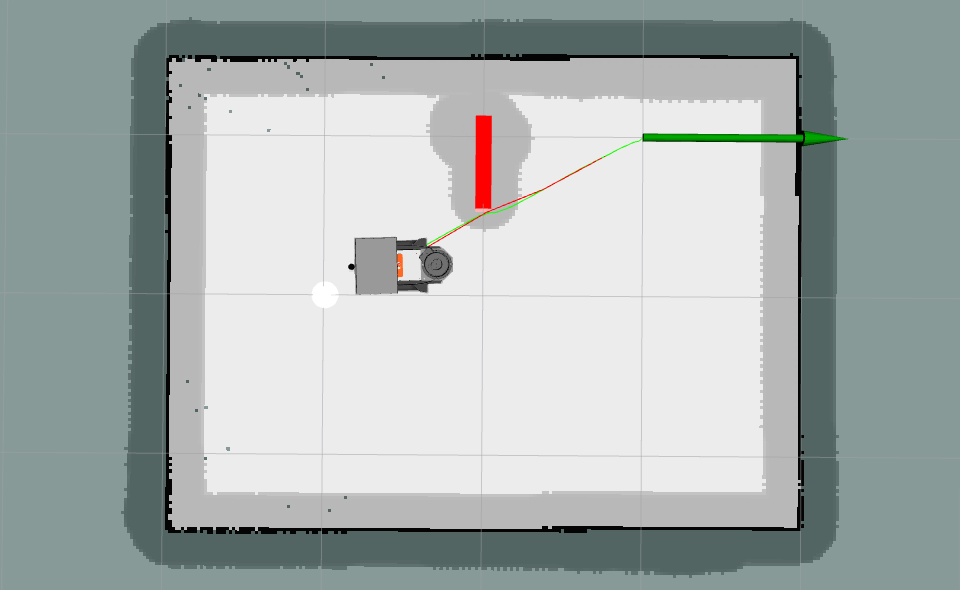
\includegraphics[width=0.95\textwidth]{images/eband_2_single_1_obs/1/5133.png} \caption{t=1.33s}
    \end{subfigure}%
    \begin{subfigure}[b]{0.30\linewidth}
        \centering
        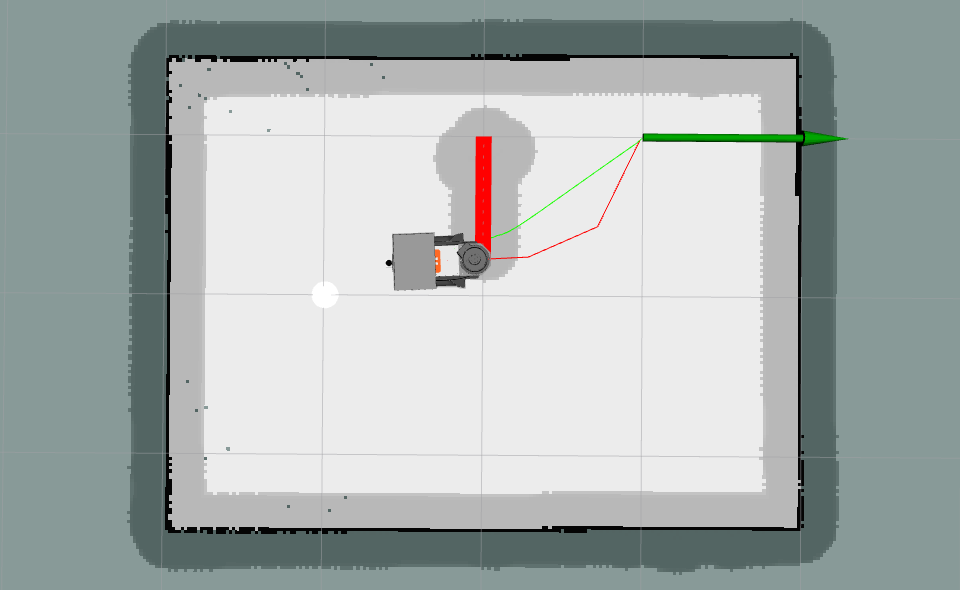
\includegraphics[width=0.95\textwidth]{images/eband_2_single_1_obs/1/5199.png} \caption{t=1.99s}
    \end{subfigure}
    \begin{subfigure}[b]{0.30\linewidth}
        \centering
        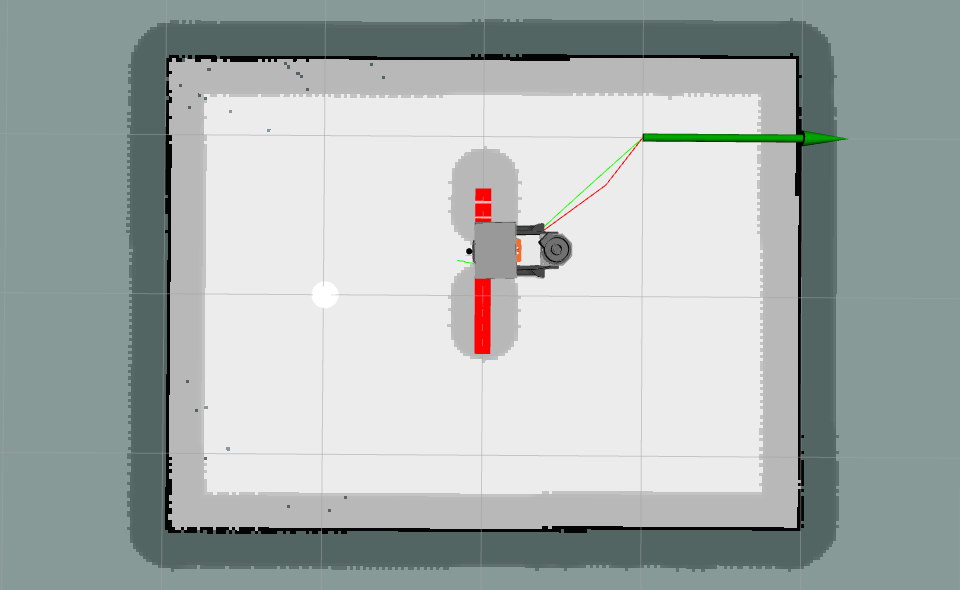
\includegraphics[width=0.95\textwidth]{images/eband_2_single_1_obs/1/5318.png} \caption{t=3.18s}
    \end{subfigure}%
    \begin{subfigure}[b]{0.30\linewidth}
        \centering
        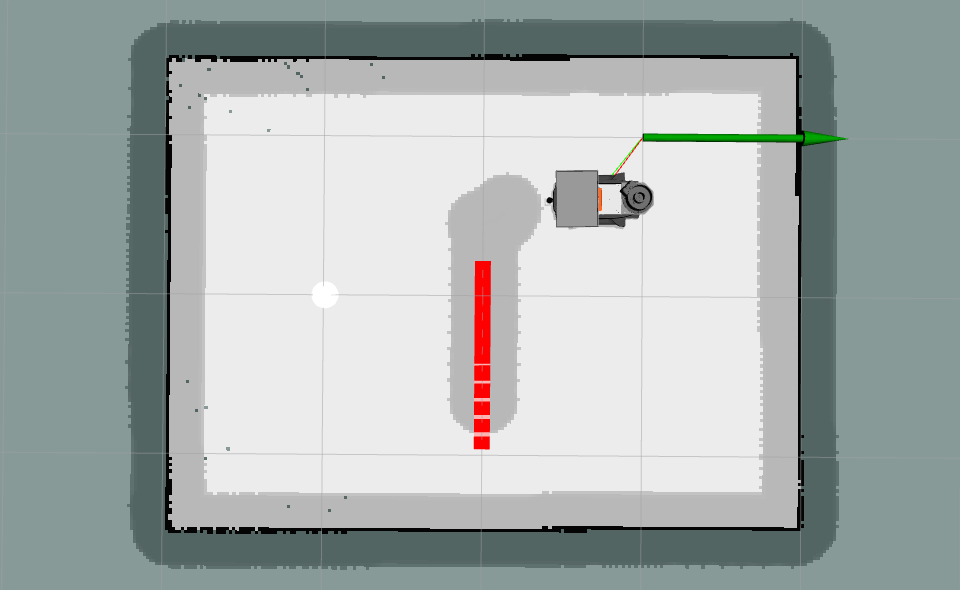
\includegraphics[width=0.95\textwidth]{images/eband_2_single_1_obs/1/5450.png} \caption{t=4.50s}
    \end{subfigure}%
    \begin{subfigure}[b]{0.30\linewidth}
        \centering
        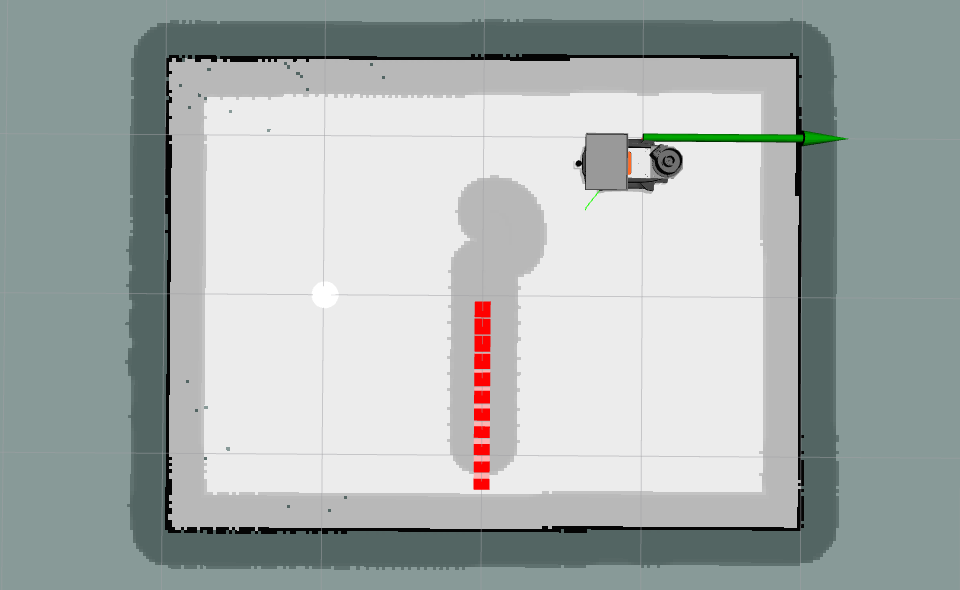
\includegraphics[width=0.95\textwidth]{images/eband_2_single_1_obs/1/5523.png} \caption{t=5.23s}
    \end{subfigure}
    \caption{EBand2 planner navigating in test case 1 (experiment 1) (green line is global path, 
    red line is Eband's plan, red squares are moving obstacle and fake obstacles created by
    \texttt{obs\_to\_costmap} and green arrow is goal)}\label{fig:eband_test_case_1_exp_1}
\end{figure}
%==================================================
\newpage{}
\section{Test case 2}%
\label{sec:test_case_2}

This test case contains an additional moving obstacle compared to test case 1. We perform 4 experiments 
starting at different time. This makes the evaluation unbiased with respect to
the starting position of the obstacles.  
Figure~\ref{fig:test_case_2_experiment_start} shows the start positions and directions of the moving
obstacles for each experiment. The trajectory and the velocity of the moving obstacle is same for each
experiment as described in~\ref{sec:test_case_2_two_obstacle_single_room}. We have included only the  
execution images for TEB local planner for this test case. However, the images are available at~\cite{evalimages}.

\begin{figure}[H]
    \centering
    \begin{subfigure}[b]{0.50\linewidth}
        \centering
        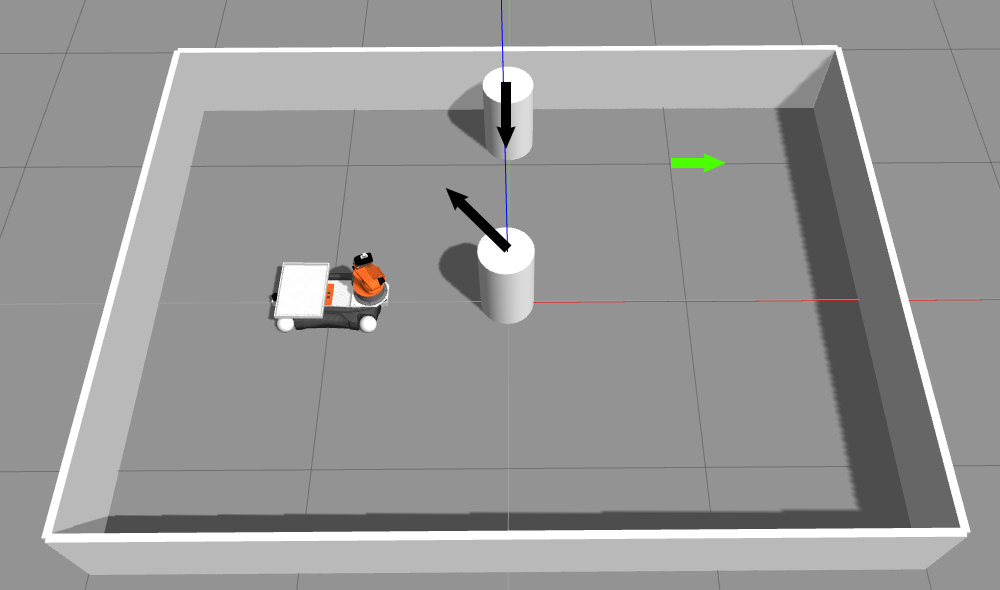
\includegraphics[width=0.95\textwidth]{images/test_case_2/exp1.png}
        \caption{Experiment 1}
    \end{subfigure}%
    \begin{subfigure}[b]{0.50\linewidth}
        \centering
        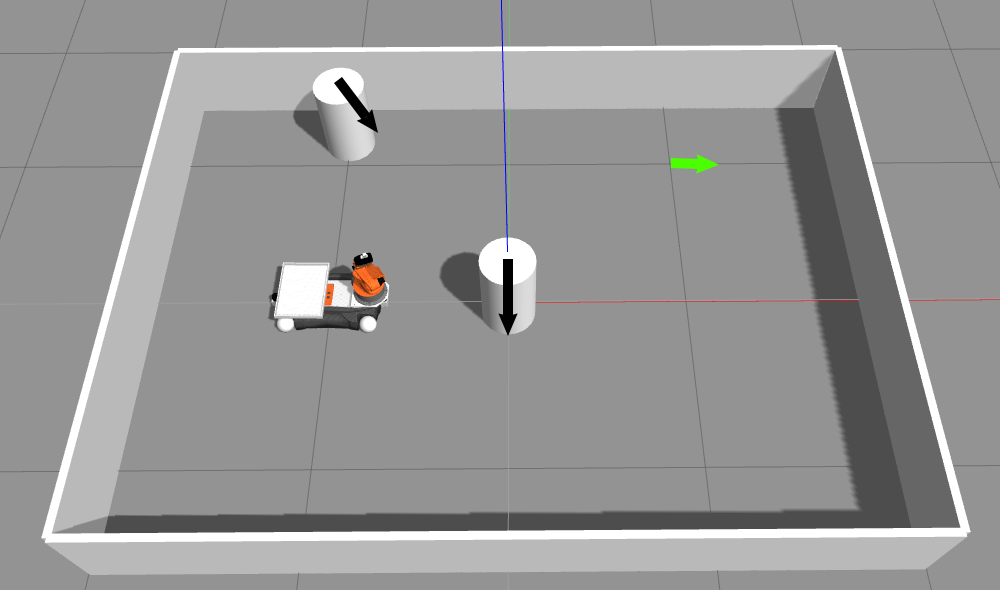
\includegraphics[width=0.95\textwidth]{images/test_case_2/exp2.png}
        \caption{Experiment 2}
    \end{subfigure}
    \begin{subfigure}[b]{0.50\linewidth}
        \centering
        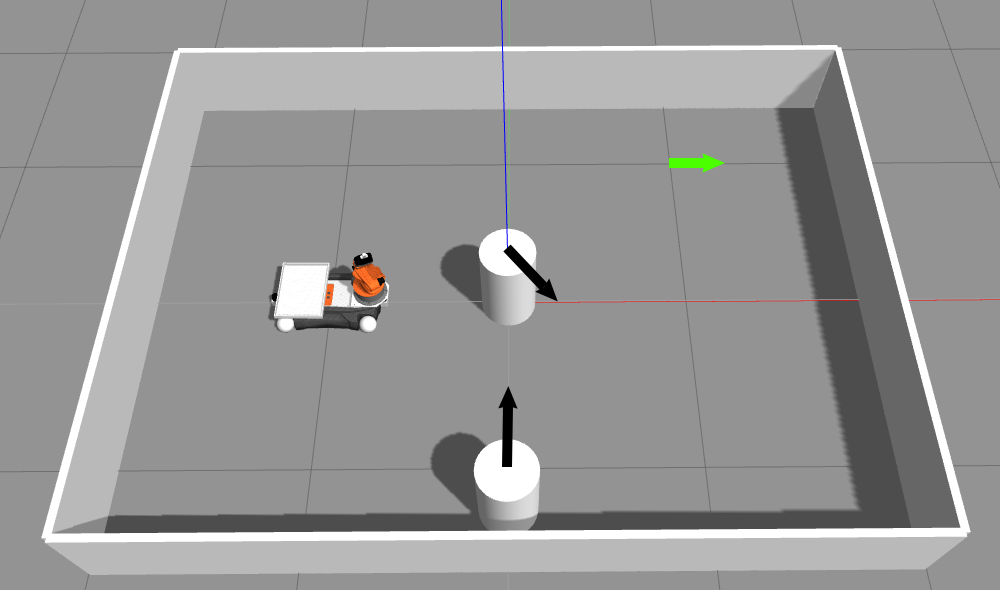
\includegraphics[width=0.95\textwidth]{images/test_case_2/exp3.png}
        \caption{Experiment 3}
    \end{subfigure}%
    \begin{subfigure}[b]{0.50\linewidth}
        \centering
        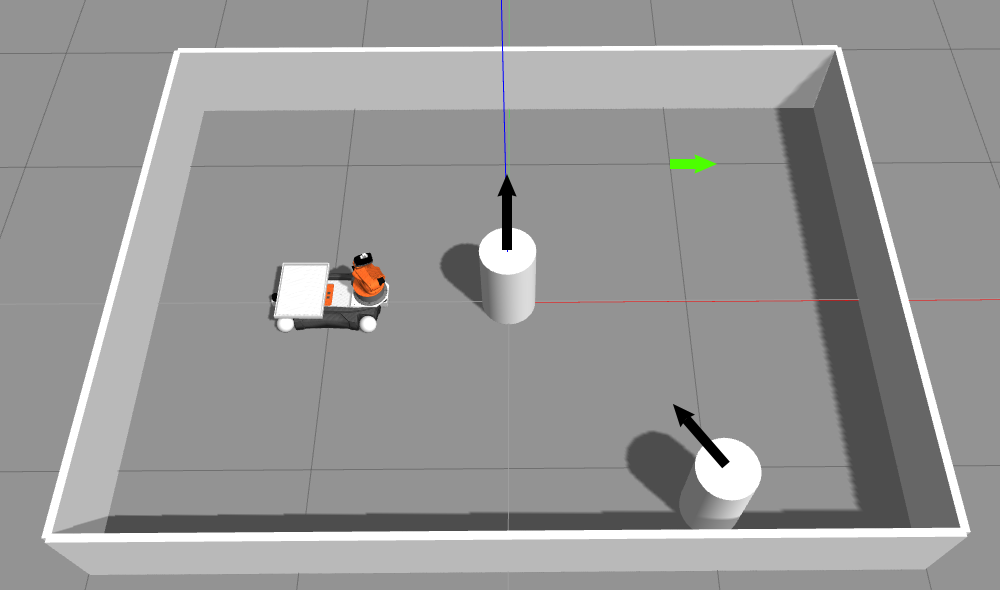
\includegraphics[width=0.95\textwidth]{images/test_case_2/exp4.png}
        \caption{Experiment 4}
    \end{subfigure}%
    \caption{Moving obstacle positions and directions (black arrow) for experiments in test case 2.
    (Green arrow is goal position and orientation)}\label{fig:test_case_2_experiment_start}
\end{figure}

\subsection{TEB local planner}%
\label{sub:eval_teb_local_planner_tc2}

\begin{table}[H]
    \centering
    \begin{tabular}{cccc}
        \textbf{Experiment} & \textbf{Travel time} & \textbf{Re-plans} & \textbf{Collisions} \\\toprule
        static & 5.205 & 0 & 0 \\
             1 & 7.381 & 1 & 0 \\
             2 & 5.097 & 0 & 0 \\
             3 & 5.400 & 0 & 0 \\
             4 & 6.454 & 1 & 0 \\
    \end{tabular}
    \caption{Performance of teb local planner navigating in test case 2}\label{tab:perfomance_teb_test_case_2}
\end{table}

\begin{figure}[H]
    \centering
    \begin{subfigure}[b]{0.35\linewidth}
        \centering
        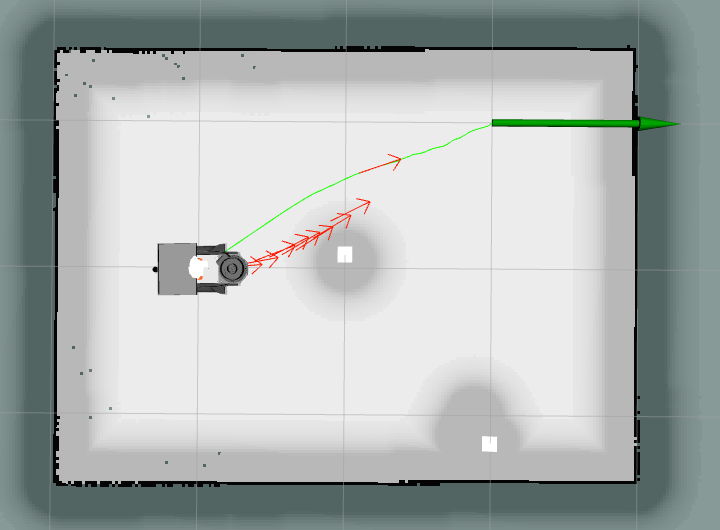
\includegraphics[width=0.95\textwidth]{images/teb_single_2_obs/4/2527.png}
        \caption{t=0.27s}
    \end{subfigure}%
    \begin{subfigure}[b]{0.35\linewidth}
        \centering
        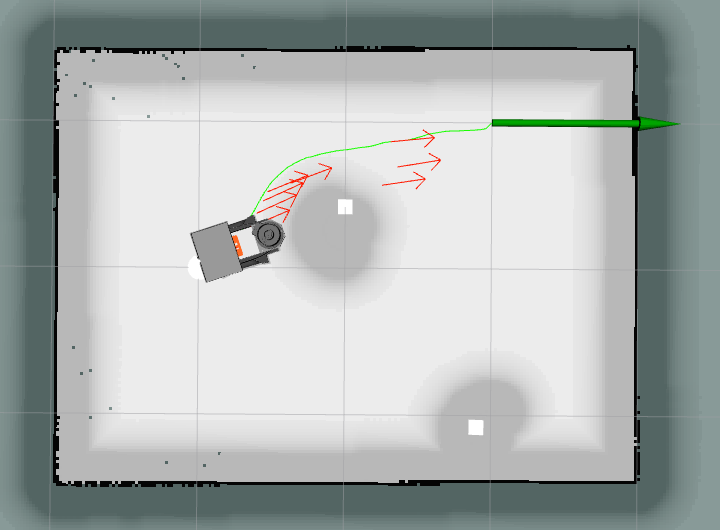
\includegraphics[width=0.95\textwidth]{images/teb_single_2_obs/4/2618.png}
        \caption{t=1.18s}
    \end{subfigure}%
    \begin{subfigure}[b]{0.35\linewidth}
        \centering
        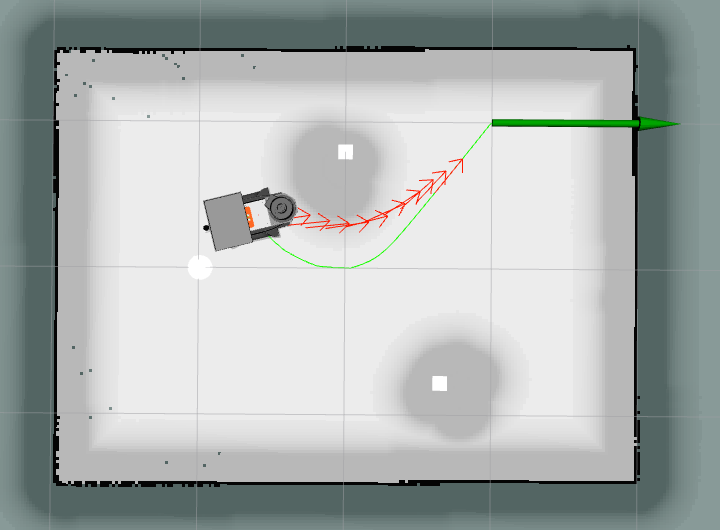
\includegraphics[width=0.95\textwidth]{images/teb_single_2_obs/4/2738.png}
        \caption{t=2.38s}
    \end{subfigure}
    \begin{subfigure}[b]{0.35\linewidth}
        \centering
        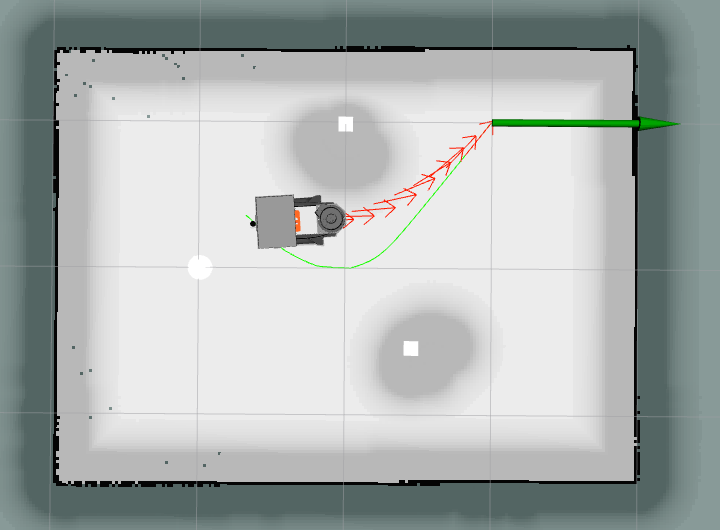
\includegraphics[width=0.95\textwidth]{images/teb_single_2_obs/4/2815.png}
        \caption{t=3.15s}
    \end{subfigure}%
    \begin{subfigure}[b]{0.35\linewidth}
        \centering
        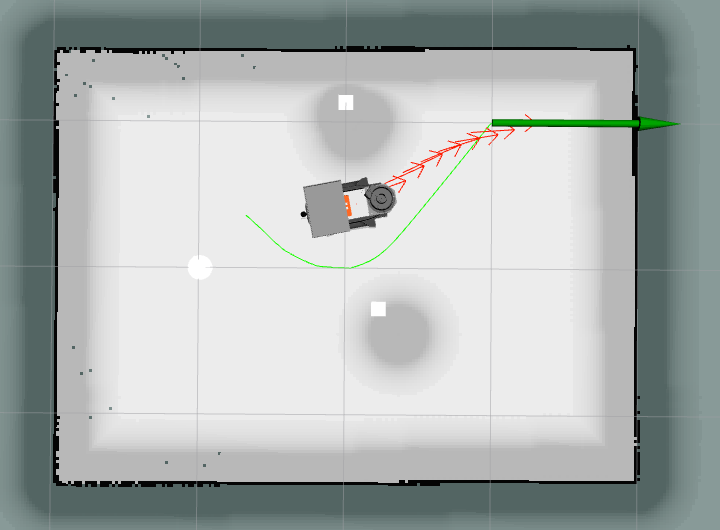
\includegraphics[width=0.95\textwidth]{images/teb_single_2_obs/4/2900.png}
        \caption{t=4.00s}
    \end{subfigure}%
    \begin{subfigure}[b]{0.35\linewidth}
        \centering
        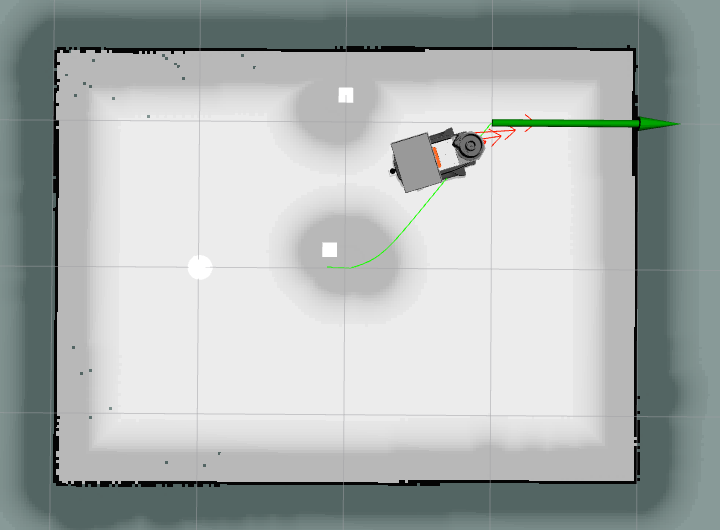
\includegraphics[width=0.95\textwidth]{images/teb_single_2_obs/4/3045.png}
        \caption{t=5.45s}
    \end{subfigure}%
    \caption{teb local planner navigating in test case 2 (experiment 4) (Line in green is
        global path, red arrows are local planner's path, green arrow is goal position and 
        white square is the obstacle)}\label{fig:teb_test_case_2_exp_4}
\end{figure}

\subsection{Spline based planner}%
\label{sub:eval_spline_based_planner_tc2}

\begin{table}[H]
    \centering
    \begin{tabular}{cccc}
        \textbf{Experiment} & \textbf{Travel time} & \textbf{Re-plans} & \textbf{Collisions} \\\toprule
        static & 5.421 & 0 & 0 \\
             1 & 6.449 & 0 & 0 \\
             2 & 5.405 & 0 & 0 \\
             3 & 5.423 & 0 & 0 \\
             4 & 6.000 & 0 & 0 \\
    \end{tabular}
    \caption{Performance of spline based planner navigating in test case 2}\label{tab:perfomance_spline_test_case_2}
\end{table}

\subsection{DWA planner}%
\label{sub:eval_dwa_planner_tc2}

\begin{table}[H]
    \centering
    \begin{tabular}{cccc}
        \textbf{Experiment} & \textbf{Travel time} & \textbf{Re-plans} & \textbf{Collisions} \\\toprule
        static & 19.526 & 0 & 0 \\
             1 & 17.773 & 0 & 0 \\
             2 & 10.877 & 0 & 0 \\
             3 & 14.046 & 0 & 0 \\
             4 & 25.760 & 2 & 2 \\
    \end{tabular}
    \caption{Performance of DWA planner navigating in test case 2}\label{tab:perfomance_dwa_test_case_2}
\end{table}

\subsection{EBand planner}%
\label{sub:eval_eband_planner_tc2}

\begin{table}[H]
    \centering
    \begin{tabular}{cccc}
        \textbf{Experiment} & \textbf{Travel time} & \textbf{Re-plans} & \textbf{Collisions} \\\toprule
        static & 6.270 & 0 & 0 \\
             1 & \-- & Failed & 2 \\
             2 & 5.590 & 0 & 0 \\
             3 & 6.242 & 0 & 0 \\
             4 & 6.887 & 1 & 0 \\
    \end{tabular}
    \caption{Performance of EBand planner navigating in test case 2}\label{tab:perfomance_eband_test_case_2}
\end{table}


\subsection{EBand2 planner}%
\label{sub:eval_eband2_planner_tc2}

\begin{table}[H]
    \centering
    \begin{tabular}{cccc}
        \textbf{Experiment} & \textbf{Travel time} & \textbf{Re-plans} & \textbf{Collisions} \\\toprule
        static & 6.270 & 0 & 0 \\
             1 & 6.933 & 1 & 0 \\
             2 & 5.952 & 0 & 0 \\
             3 & 5.694 & 0 & 0 \\
             4 & 6.355 & 1 & 0 \\
    \end{tabular}
    \caption{Performance of EBand2 planner navigating in test case 2}\label{tab:perfomance_eband2_test_case_2}
\end{table}

%==================================================
\newpage{}
\section{Test case 3}%
\label{sec:test_case_3}

There are 2 rooms connected by a corridor in this test case environment. We perform 4 experiments 
starting at different time. This makes the evaluation unbiased with respect to
the starting position of the obstacles. The moving obstacles are all in sync in terms of velocity. 
They all stop at the same time and have a highest velocity at the same time.   
Figure~\ref{fig:test_case_3_experiment_start} shows the start positions and directions of the moving
obstacles for each experiment. The trajectory and the velocity of the moving obstacle is same for each
experiment as described in~\ref{sec:test_case_3_double_room}. We have included the images for the 
execution of TEB local planner only, images for other execution are available at~\cite{evalimages}.

\begin{figure}[H]
    \centering
    \begin{subfigure}[b]{0.50\linewidth}
        \centering
        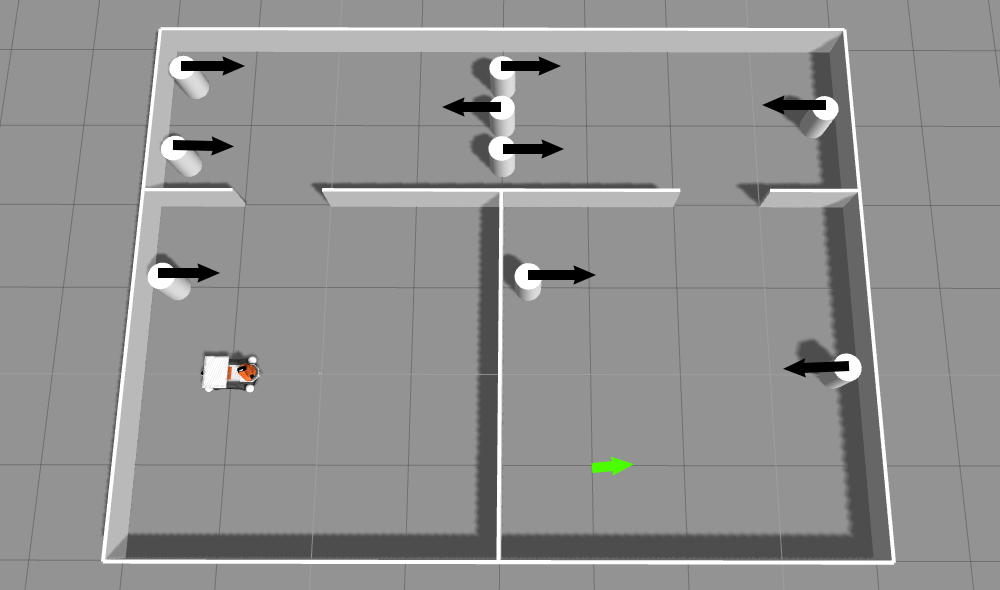
\includegraphics[width=0.95\textwidth]{images/test_case_3/exp1.png}
        \caption{Experiment 1}
    \end{subfigure}%
    \begin{subfigure}[b]{0.50\linewidth}
        \centering
        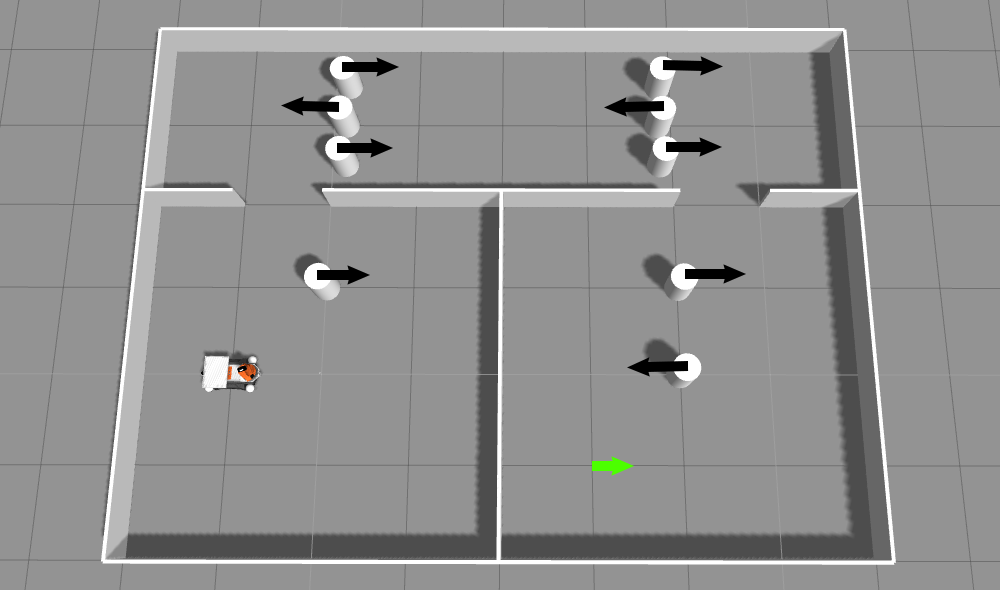
\includegraphics[width=0.95\textwidth]{images/test_case_3/exp2.png}
        \caption{Experiment 2}
    \end{subfigure}
    \begin{subfigure}[b]{0.50\linewidth}
        \centering
        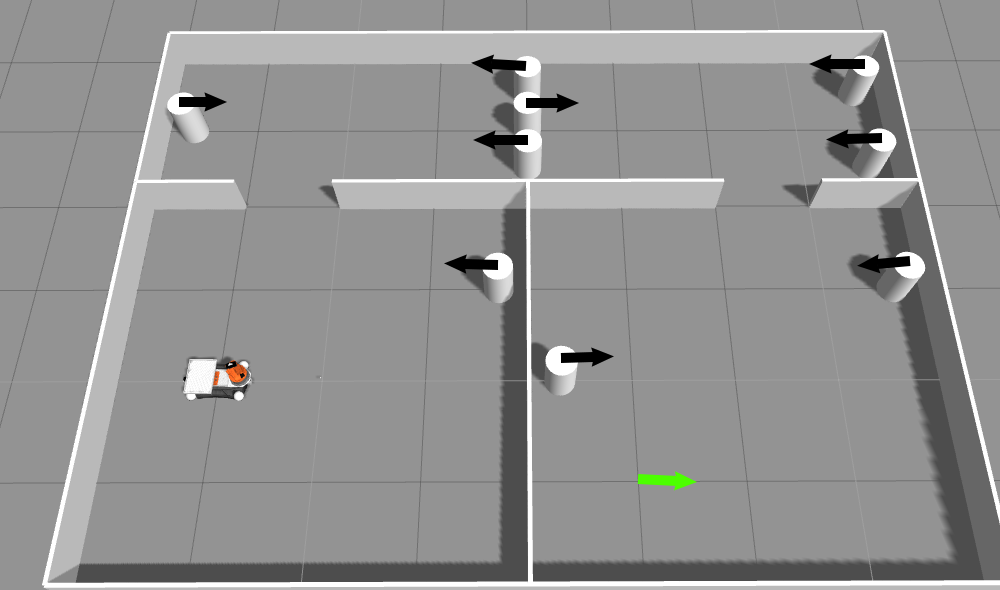
\includegraphics[width=0.95\textwidth]{images/test_case_3/exp3.png}
        \caption{Experiment 3}
    \end{subfigure}%
    \begin{subfigure}[b]{0.50\linewidth}
        \centering
        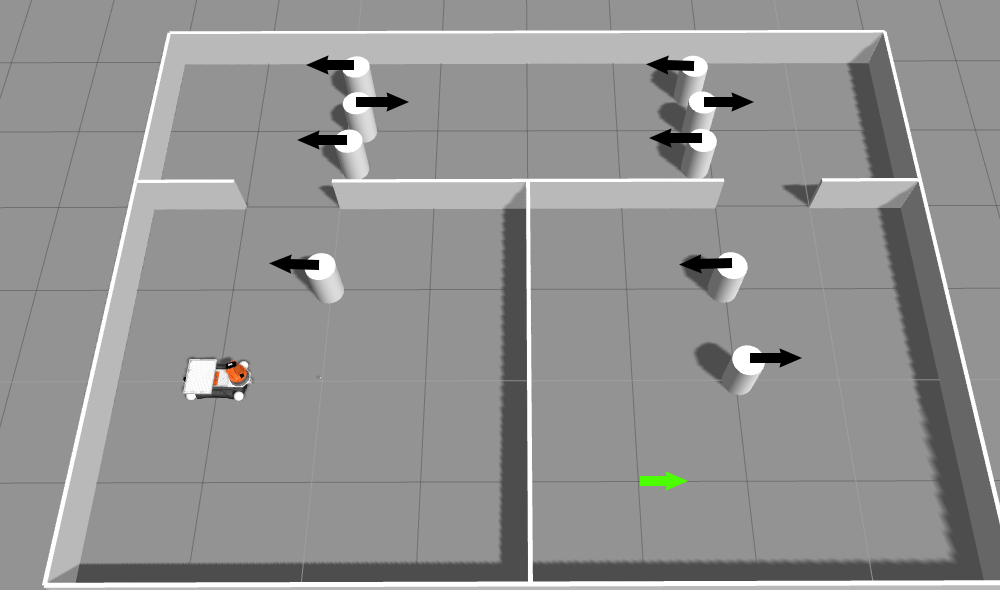
\includegraphics[width=0.95\textwidth]{images/test_case_3/exp4.png}
        \caption{Experiment 4}
    \end{subfigure}
    \caption{Moving obstacle positions and directions (black arrow) for experiments in test case 3.
    (Green arrow is goal position and orientation)}\label{fig:test_case_3_experiment_start}
\end{figure}

\subsection{TEB local planner}%
\label{sub:eval_teb_local_planner_tc3}

\begin{table}[H]
    \centering
    \begin{tabular}{cccc}
        \textbf{Experiment} & \textbf{Travel time} & \textbf{Re-plans} & \textbf{Collisions} \\\toprule
        static & 27.139 & 0 & 0 \\
             1 & 37.399 & 4 & 0 \\
             2 & 27.204 & 2 & 0 \\
             3 & 40.229 & 4 & 1 \\
             4 & 36.487 & 3 & 2 \\
    \end{tabular}
    \caption{Performance of teb local planner navigating in test case 3}\label{tab:perfomance_teb_test_case_3}
\end{table}

\begin{figure}[!ht]
    \centering
    \begin{subfigure}[b]{0.35\linewidth}
        \centering
        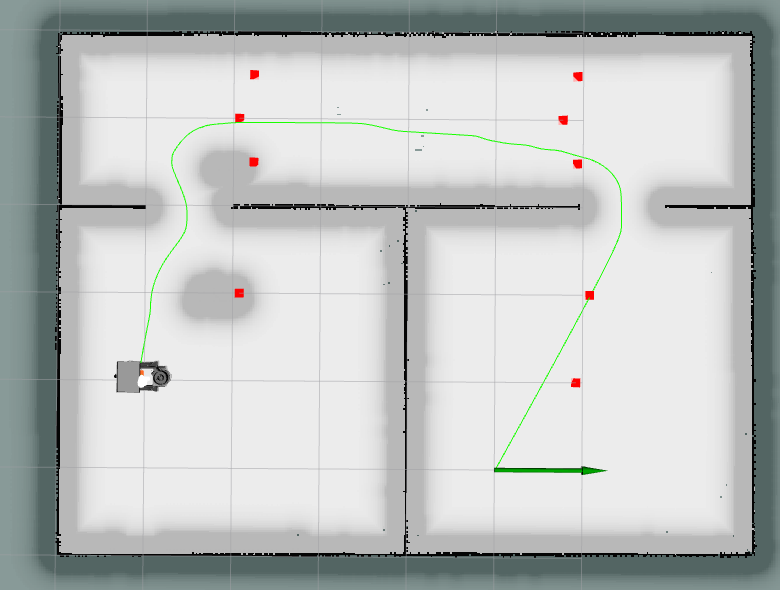
\includegraphics[width=0.95\textwidth]{images/teb_double/2/772.png} \caption{t=0.22s}
    \end{subfigure}%
    \begin{subfigure}[b]{0.35\linewidth}
        \centering
        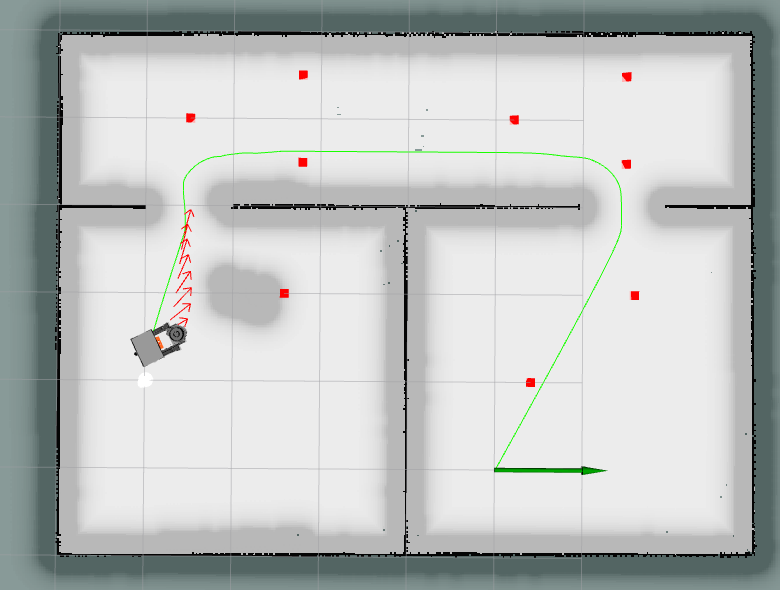
\includegraphics[width=0.95\textwidth]{images/teb_double/2/927.png} \caption{t=1.77s}
    \end{subfigure}%
    \begin{subfigure}[b]{0.35\linewidth}
        \centering
        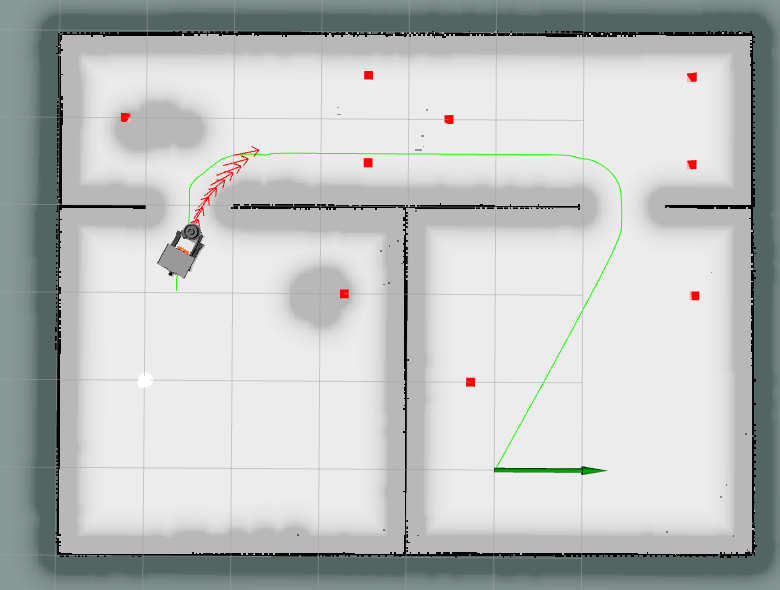
\includegraphics[width=0.95\textwidth]{images/teb_double/2/1170.png} \caption{t=4.20s}
    \end{subfigure}
    \begin{subfigure}[b]{0.35\linewidth}
        \centering
        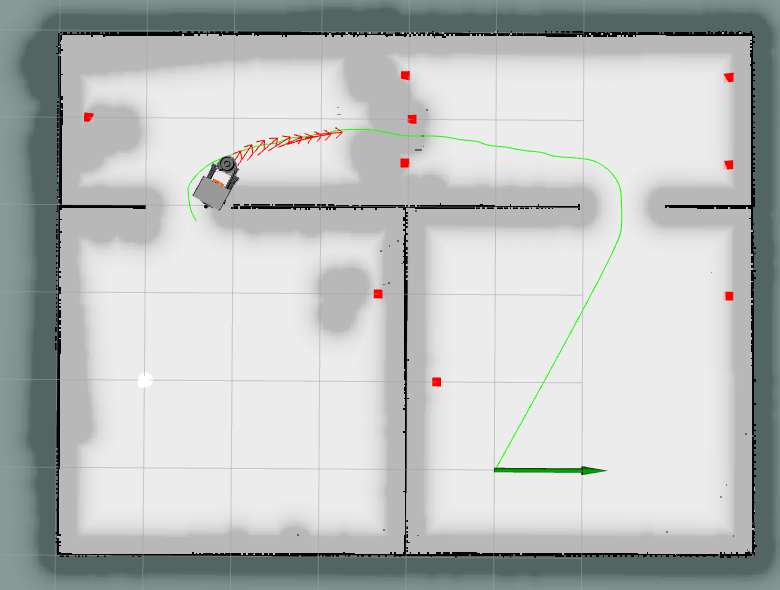
\includegraphics[width=0.95\textwidth]{images/teb_double/2/1408.png} \caption{t=6.58s}
    \end{subfigure}%
    \begin{subfigure}[b]{0.35\linewidth}
        \centering
        \includegraphics[width=0.95\textwidth]{images/teb_double/2/1607.png} \caption{t=8.57s}
    \end{subfigure}%
    \begin{subfigure}[b]{0.35\linewidth}
        \centering
        \includegraphics[width=0.95\textwidth]{images/teb_double/2/1949.png} \caption{t=11.99s}
    \end{subfigure}
    \begin{subfigure}[b]{0.35\linewidth}
        \centering
        \includegraphics[width=0.95\textwidth]{images/teb_double/2/2388.png} \caption{t=16.38s}
    \end{subfigure}%
    \begin{subfigure}[b]{0.35\linewidth}
        \centering
        \includegraphics[width=0.95\textwidth]{images/teb_double/2/2519.png} \caption{t=17.69s}
    \end{subfigure}%
    \begin{subfigure}[b]{0.35\linewidth}
        \centering
        \includegraphics[width=0.95\textwidth]{images/teb_double/2/2826.png} \caption{t=20.76s}
    \end{subfigure}
    \begin{subfigure}[b]{0.35\linewidth}
        \centering
        \includegraphics[width=0.95\textwidth]{images/teb_double/2/3201.png} \caption{t=24.51s}
    \end{subfigure}%
    \begin{subfigure}[b]{0.35\linewidth}
        \centering
        \includegraphics[width=0.95\textwidth]{images/teb_double/2/3466.png} \caption{t=27.16s}
    \end{subfigure}%
    \begin{subfigure}[b]{0.35\linewidth}
        \centering
        \includegraphics[width=0.95\textwidth]{images/teb_double/2/3711.png} \caption{t=04.91s}
    \end{subfigure}
    \caption{teb local planner navigating in test case 3 (experiment 2) (Line in green is
    global path, red arrows are local planner's path and red square is the obstacle)}\label{fig:teb_test_case_3_exp_2}
\end{figure}

\subsection{Spline based planner}%
\label{sub:eval_spline_based_planner_tc3}
Spline based planner has its own method for combining global planner with the local motion planner.
It uses iterative method to form a rectangular area around the robot as large as possible. It then
gets a global plan (using A* algorithm) inside this region. The local planner uses this information
to create a smooth and collision free path. This method works in the planner's simulator, however the
parameters are extremely sensitive for the planner to work correctly (as of yet). When combined with ROS framework,
this method does not work because the current method is only configured for a circular and very small
robot navigating in a relatively large environment. The method fails completely in narrow passages. 
In test case 3, we have 2 narrow spaces (doorways) with static obstacles alone. We tried to combine the motion
planner with their global planner in a simple way where the motion planner can only change trajectory between 2 global
waypoints. The motion planner still fails at the narrow regions (even in a static environment).

\begin{table}[H]
    \centering
    \begin{tabular}{cccc}
        \textbf{Experiment} & \textbf{Travel time} & \textbf{Re-plans} & \textbf{Collisions} \\\toprule
        static & \-- & Failed & 0 \\
             1 & \-- & Failed & 0 \\
             2 & \-- & Failed & 0 \\
             3 & \-- & Failed & 0 \\
             4 & \-- & Failed & 0 \\
    \end{tabular}
    \caption{Performance of spline based planner navigating in test case 3}\label{tab:perfomance_spline_test_case_3}
\end{table}

\subsection{DWA planner}%
\label{sub:eval_dwa_planner_tc3}

As shown in Table~\ref{tab:perfomance_teb_test_case_3}, DWA planner is able to successfully navigate
in static environment in less than 40 seconds. However, planner fails completely while travelling
through the corridor. We expected this because of the \texttt{lookahead\_time} being not optimal
for this scenario as mentioned in~\ref{sec:obstacle_trajectory_to_costmap}. As shown in Figure~\ref{fig:blocked_planner_in_corridor},
the complete corridor is believed to be occupied by the planner. Even if the planner did not give up,
it will almost always perceive the corridor to be untraversable.

\begin{table}[H]
    \centering
    \begin{tabular}{cccc}
        \textbf{Experiment} & \textbf{Travel time} & \textbf{Re-plans} & \textbf{Collisions} \\\toprule
        static & 39.004 & 0 & 0 \\
             1 & \-- & Failed & 2 \\
             2 & \-- & Failed & \-- \\
             3 & \-- & Failed & \-- \\
             4 & \-- & Failed & \-- \\
    \end{tabular}
    \caption{Performance of DWA planner navigating in test case 1}\label{tab:perfomance_dwa_test_case_3}
\end{table}

\begin{figure}[H]
    \centering
    \includegraphics[width=0.5\linewidth]{images/dwa_double/1/fail.png}
    \caption{\label{fig:blocked_planner_in_corridor} Robot's path completely blocked by obstacles and 
        fake obstacles created by obs\_to\_costmap}
\end{figure}

\subsection{EBand planner}%
\label{sub:eval_eband_planner_tc3}

\begin{table}[H]
    \centering
    \begin{tabular}{cccc}
        \textbf{Experiment} & \textbf{Travel time} & \textbf{Re-plans} & \textbf{Collisions} \\\toprule
        static & 30.862 & 0 & 0 \\
             1 & 76.982 & 8 & 6 \\
             2 & 71.808 & 7 & 2 \\
             3 & \-- & Failed & 3 \\
             4 & 67.113 & 4 & 5 \\
    \end{tabular}
    \caption{Performance of EBand planner navigating in test case 3}\label{tab:perfomance_eband_test_case_3}
\end{table}


\subsection{EBand2 planner}%
\label{sub:eval_eband2_planner_tc3}

Similar to DWA, EBand2 uses \texttt{obs\_to\_costmap}. The results are pretty much same except that 
EBand2 planner does not reach as far and returns failure very early if it does not find a path.

\begin{table}[H]
    \centering
    \begin{tabular}{cccc}
        \textbf{Experiment} & \textbf{Travel time} & \textbf{Re-plans} & \textbf{Collisions} \\\toprule
        static & 30.862 & 0 & 0 \\
             1 & \-- & Failed & \-- \\
             2 & \-- & Failed & \-- \\
             3 & \-- & Failed & 1 \\
             4 & \-- & Failed & \-- \\
    \end{tabular}
    \caption{Performance of EBand2 planner navigating in test case 3}\label{tab:perfomance_eband2_test_case_3}
\end{table}

